\documentclass[10pt,twoside,draft]{memoir}

\usepackage{salitter}
\usletterlayout

\usepackage{mwe}
\usepackage{amsmath}
\usepackage{stix}
\usepackage{xfrac}
\usepackage{bbold}
\usepackage{csquotes}
\usepackage[normalem]{ulem}
\usepackage{enumitem}

% fonts
\newpxfont

\newcommand{\tocline}{
	\addtocontents{toc}{\protect\mbox{}\protect\hrulefill\par}}
\setlength\cftbeforepartskip{1.1em}
\setlength\cftbeforechapterskip{0.5em}

\renewcommand{\printpartname}{}
\renewcommand{\parttitlefont}{\normalfont\Huge\scshape}

% \usepackage{cabin}
% \newfontfamily{\specialheadersfont}{Cabin}

\newcommand{\speech}[1]{
	\textquote{\emph{#1}}}

\newcommand{\said}[1]{ % oops
	\speech{#1}}

\newcommand{\essaytitle}[1]{\uline{#1}}

\newcommand{\gap}{\plainbreak{2}}

\newcommand{\inlineaside}[1]{\textit{(#1)}}

\newcommand{\x}{$x$}
\newcommand{\y}{$y$}

\newcommand{\redact}[1]{\xout{#1}}

\newcommand{\greater}{>}
\newcommand{\less}{<}

% TODO because of something tricky ill need to debug later
\newcommand{\bimg}[1]{(img #1)}

% --- typesetting aids for some subtle syntax of flynt
\newcommand{\formulation}[1]{'\textit{#1}'}

\newcommand{\triquote}[1]{'''#1'''}

% TODO these should be considered placeholders basically
\newcommand{\name}[1]{\textbf{#1}}

% "linguistic expression"
\newcommand{\lexpression}[1]{"\emph{#1}"}
\newcommand{\expression}[1]{\lexpression{#1}}

\newenvironment{sysrules}{
	\begin{hangparas}{3em}{1}
	}{
	\end{hangparas}
	}

\newcommand{\postulate}[1]{
	\emph{Postulate #1}.}

\newcommand{\dreamdate}[1]{
	\plainbreak{1} \uline{#1}\\ }
\newcommand{\dreamdatecomment}[2]{
	\plainbreak{1} \uline{#1} --- \textit{#2}\\ }

\newcommand{\cubeframe}{
	
\includegraphics[width=1em]{img/cubeframe}}
\newcommand{\cubeup}{
	
\includegraphics[width=1em]{img/cubeup}}
\newcommand{\cubedown}{
	
\includegraphics[width=1em]{img/cubedown}}

\begin{document}
\frontmatter
\graphicspath{{img/}}
\pagestyle{ruled}
\chapterstyle{tandh}
\openany

\renewcommand*{\cftpartfont}{\bfseries\scshape}
\renewcommand*{\cftchapterfont}{\normalfont}
\renewcommand*{\cftsectionfont}{\itshape}
% \setlength\beforechapskip{10pt}
\renewcommand*{\chapterheadstart}{\vskip 1pt}


\setlist{itemsep=3pt}
\setlist{parsep=0pt}
\setlist{topsep=3pt}
\setlist{leftmargin=1cm}

% Title
\thispagestyle{empty}
{
	\centering\sffamily

	\plainbreak{3}

	{ \Large
	Blueprint for a Higher Civilization \par}

	\plainbreak{3}

	{ \large Henry Flynt \par}
}

\clearpage

\newcommand{\photopage}[3]{
	\begin{figure}[!hp]
		\centering
		\includegraphics[width=4in]{#1}
		\caption{#2 (photo by #3)}
	\end{figure}}

\photopage{img/creep}{Henry Flynt presents "Creep" lecture in Adam Hovre upper common room, Harvard University, May 15, 1962}{Tony Conrad}

\chapter{Introduction}

This essay is the third in a series on the rationale of my career. It 
summarizes the results of my activities, the consistent outlook on a whole 
range of questions which I have developed. The first essay, 
\essaytitle{On Social Recognition}, noted that the official social philosophy of practically every 
regime in the world says that the individual has a duty to serve society to the 
best of his abilities. Social recognition is supposed to be the reward which 
indicates that the individual is indeed serving society. Now it happens that 
the most important tasks the individual can undertake are tasks (intellectual, 
political, and otherwise) posed by society. However, when the individual 
undertakes such tasks, society's actual response is almost always persecution 
(Galileo) or indifference (Mendel). Thus, the doctrine that the'individual has 
a duty to serve society is a hypocritical fraud. I reject every social 
philosophy which contains this doctrine. The rational individual will obtain 
the means of subsistence by the most efficient swindle he can find. Beyond 
this, he will undertake the most important tasks posed by society for his 
own private gratification. He will not attempt to benefit society, or to gain 
the recognition which would necessarily result if society were to utilize his 
achievements. 

The second essay, \essaytitle{Creep}, discussed the practices of isolating oneself; 
carefully controlling one's intake of ideas and influences from outside; and 
playing as a child does. I originally saw these practices as the effects of 
certain personality problems. However, it now seems that they are actually 
needed for the intellectual approach which I have developed. They may be 
desirable in themselves, rather than being mere effects of personality 
problems. 

I chose fundamental philosophy as my primary subject of investigation. 
Society presses me to accept all sorts of beliefs. At one time it would have 
pressed me to believe that the earth was flat; then it reversed itself and 
demanded that I believe the earth is round. The majority of Americans still 
consider it "necessary" to believe in God; but the Soviet government has 
managed to function for decades with an atheistic philosophy. Thus, which 
beliefs should I accept? My analysis is presented in writings entitled 
\essaytitle{Philosophy Proper}, \essaytitle{The Flaws Underlying Beliefs}, and 
\essaytitle{Philosophical Aspects of Walking Through Walls}. 
The question of whether a given belief is valid 
depends on the issue of whether there is a realm beyond my "immediate 
experience." Does the Empire State Building continue to exist even when I 
am not looking at it? If such a question can be asked, there must indeed be 
a realm beyond my experience, because otherwise the phrase 'a realm 
beyond my experience' could not have any meaning. (Russell's theory of 
descriptions does not apply in this case.) But if the assertion that there is a 
realm beyond my experience is true merely because it is meaningful, it 
cannot be substantive; it must be a definitional trick. In general, beliefs 
depend on the assertion of the existence of a realm beyond my experience, 
an assertion which is nonsubstantive. Thus, beliefs are nonsubstantive or 
meaningless; they are definitional tricks. Psychologically, when I believe that 
the Empire State Building exists even though I am not looking at it, I 
imagine the Empire State Building, and I have the attitude toward this 
mental picture that it is a perception rather than a mental picture. The 
attitude involved is a self-deceiving psychological trick which corresponds to 
the definitional trick in the belief assertion. The conclusion is that all beliefs 
are inconsistent or self-deceiving. It would be beside the point to doubt 
beliefs, because whatever their connotations may be, logically beliefs are 
nonsense, and their negations are nonsense also. 

The important consequence of my philosophy is the rejection of truth 
as an intellectual modality. I conclude that an intellectual activity's claim to 
have objective value should not depend on whether it is true; and also that 
an activity may perfectly weil employ false statements and still have 
objective value. I have developed activities which use mental capabilities that 
are excluded by a truth-oriented approach: descriptions of imaginary 
phenomena, the deliberate adoption of false expectations, the thinking of 
contradictions, and meanings which are reversed by the reader's mental 
reactions; as well as illusions, the deliberate suspension of normal beliefs, and 
phrases whose meaning is stipulated to be the associations they evoke. It 
must be clear that these activities are not in any way whatever a return to 
pre-scientific trrationalism. My philosophy demolishes astrology even more 
than it does astronomy. The irrationalist is out to deceive you; he wants you 
to believe that his superstitions are truths. My activities, on the other hand, 
explicitly state that they are using non-true material. My intent is not to get 
you to believe that superstitions are truths, but to exploit non-true material 
for rational purposes. 

The other initial subject of investigation I chose was art. The art which 
claims to have cognitive value is already demolished by my philosophical 
results. However, art at its most distinctive does not need to claim cognitive 
value; its value is claimed to be entertainmental or amusemental. What about 
art whose justification is simply that people like it? Consider things which 
are just liked, or whose value is purely subjective. I point out that each 
individual already has experiences, prior to art, whose value is purely 
subjective. (Call these experiences "brend.") The difference between brend 
and art is that in art, the thing valued is separated from the valuing of it and 
turned into an object which is urged on other people. Individuals tend to 
overlook their brend, and they do so because of the same factors which 
perpetuate art. These factors include the relation between the socialization 
of the individual and the need for an escape from work. The conditioning 
which causes one to venerate "great art" is also a conditioning to dismiss 
one's own brend. If one can become aware of one's brend without the 
distortion produced by this conditioning, one finds that one's brend is 
superior to any art, because it has a level of personalization and originality 
which completely transcends art. 

Thus, I reject art as an intellectual or cultural modality. In rejecting 
truth, I advocated in its place intellectual activities which have an objective 
value independent of truth. In rejecting art, I do not propose that it be 
replaced with any objective activity at all. Rather, I advocate that the 
individual become aware of his just-likings for what they are, and allow them 
to come out. If I succeed in getting the individual to recognize his own 
just-likings, then I will have given him infinitely more than any artist ever 
can. 

We are not finished with art, however. Ever since art began to 
disintegrate as an institution, modern art has become more and more of a 
repository for activities which represent pure waste, but which counterfeit 
innovation and objective value. A two-way process is involved here. On the 
one hand, the modern artist, faced with the increasing gratuitousness of his 
profession, desperately incorporates superficial references to science in his 
products in the hope of intimidating his audience. On the other hand, art 
itself has become an institution which invests waste with legitimacy and even 
prestige; and it offers instant rewards to people who wish to play the game. 
What is innovation in modern art? You take a poem by Shelly, cut it up into 
little pieces, shake the pieces up in a box, then draw them out and write 
down whatever is on them in the order in which they are drawn. If you call 
the result a "modern poem," people will suddenly be awed by it, whereas 
they would not have been awed otherwise. This sort of innovation is utterly 
mechanical and superficial. When artists incorporate scientific references in 
their products, the process is similarly a mechanical, superficial 
amalgamation of routine artistic material with current gadgets. 

Now there may be some confusion as to what the difference is between 
the products which result from this attempt to "save" art, and activities in 
the intellectual modality which I favor. There may be a tendency to confuse 
activities which are neither science nor art, but have objective value, with art 
products which are claimed to be "scientific" and therefore objectively 
valuable. To dispel this confusion, the following questions may be asked 
about art products. 
\begin{enumerate}
\item If the product were not called art, would it immediately be seen to be 
worthless? Does the product rely on artistic institutions to "carry" it? 

\item Suppose that the artist claims that his product embodies major scientific 
discoveries, as in the case of a ballet dancer who claims to be working in the 
field of antigravity ballet. If the dancer really has an antigravity device, 
why can it only work in a ballet theater? Why can it 
only be used to make dancers jump higher? Why do you have to be able to 
perform "Swan Lake" in order to do antigravity experiments? 
\end{enumerate}
To use a phrase from medical research, I contend that a real scientist would seek to 
isolate the active principle---not to obscure it with non-functional mumbo-jumbo. 

Both of these sets of questions make the same point, from somewhat 
different perspectives. Given an individual with a product to offer, does he 
actively seek out the lady art reporters, the public relations contracts, the 
museum officials, or does he actively dissociate himself from them? Does he 
seek artistic legitimation of his product, or does he reject it? The objective 
activities which I have developed stand on their own feet. They are not art, 
and to construe them as art would make it impossible to comprehend them. 

A definition of the intellectual modality which I favor is now in order. 
Until now, this modality has involved the construction of ideas such that the 
very possibility of thinking these ideas is a significant phenomenon. In other 
words, the modality has consisted of the invention of mental abilities. The 
ideas involve physical language, that is, language which occurs in beliefs 
about the physical world. Such language is philosophically meaningless, but 
it has connotations provided by the psychological trick involved in believing. 
The connotations are what are utilized; factual truth is irrelevant. Then, the 
ideas cannot be reduced to the mechanical manipulation of marks or 
counters---unlike ordinary mathematics. Also, logical truth, which happens to 
be discredited by my philosophical results, is irrelevant to the ideas. 

But the defining requirement of the modality is that each activity in it 
must have objective value. The activity must provide one with something 
which is useful irrespective of whether one likes it; that is, which is useful 
independently of whether it produces emotional gratification. 

We can now consider the following principle. "spontaneously and 
without any prompting to sweep human culture aside and to carry out 
elaborate, completely self-justifying activities." Relative to the social context 
of the individual's activities, this principle is absurd. We have no reason to 
respect the eccentric hobbyist, or the person who engages in arbitrary 
antisocial acts. If an action is to have more than merely personal significance, 
it must have a social justification, as is explained in On Social Recognition. 
In the light of The Flaws Underlying Beliefs and the brend theory, however, 
the principle mentioned above does become valid when it is interpreted 
correctly, because it becomes necessary to invent ends as well as means. The 
activity must provide an objective value, but this value will no longer be 
standardized. 

The modality I favor is best exemplified by \essaytitle{Energy Cube Organism},
\essaytitle{Concept Art}, and the \essaytitle{Perception-Dissociator Model}. 
\essaytitle{Energy Cube Organism} is a perfect example of ideas such that the very 
possibility of thinking them is a significant phenomenon. It is also a perfect example of an 
activity which is useful irrespective of whether it provides emotional 
gratification. It combines the description of imaginary physical phenomena 
with the thinking of contradictions. It led to \essaytitle{Studies in Constructed 
Memories}, which in turn led to \essaytitle{The Logic of Admissible Contradictions}.
With this last writing, it becomes obvious that the activity has applications 
outside itself. 

\essaytitle{Concept Art}\footnote{published in An Anthology ed. LaMonte Young, 1963}
uses linguistic expressions which are changed by the reader's mental 
reactions. It led to \essaytitle{Post-Formalism in Constructed Memories}, and this led 
in turn to \essaytitle{Subjective Propositional Vibration}.

The \essaytitle{Perception-Dissociator Model}\footnote{published in I-KON, Vol. 1, No. 5} 
was intended to exploit the realization that humans are the most 
advanced machines (or technology) that we have. I wanted to build a model 
of a machine out of humans, using a minimum of non-human props. Further, 
the machine modelled was to have capabilities which are physically 
impossible according to present-day science. I still think that the task as I 
have defined it is an excellent one; but the model does not yet completely 
accomplish the objective. The present model uses the deliberate suspension 
of normal beliefs to produce its effects. 

\essaytitle{Post-Formalism in Constructed Memories} and \essaytitle{Studies in 
Constructed Memories} together make up \booktitle{Mathematical Studies} (1966). In 
this monograph, the emphasis was on extending the idea of mathematics as 
formalistic games to games involving subjectivity and contradiction. In two 
subsequent monographs, the material was developed so as to bring out its 
potential applications in conjunction with science. 
\essaytitle{Subjective Propositional Vibration} investigates the logical 
possibilities of expressions which are changed by the reader's mental responses.
\essaytitle{The Logic of Admissible Contradictions} starts with the experiences 
of the logically impossible which 
we have when we suffer certain perceptual illusions. These illusions enable us 
to imagine certain logical impossibilities just as clearly as we imagine the 
logically possible. The monograph models the content of these illusions to 
obtain a system of logic in which some (but not all) contradictions are 
"admissible." The theory investigates the implications of admitting some 
contradictions for the admissibility of other contradictions. A theory of 
many-valued numbers is also presented. 

The \essaytitle{Perception-Dissociator Model} led to 
\essaytitle{The Perception-Dissociation of Physics.} Again, here is an essay whose 
significance lies in the very possibility of thinking the ideas at all. The essay 
defines a change in the pattern of experience which would make it 
impossibie for physicists to "construct the object from experience." Finally, 
\essaytitle{Mock Risk Games} is the activity which involves the deliberate adoption of 
false expectations. It is on the borderline of the intellectual modality which I 
favor, because it seems to me to have objective value, and yet has not 
generated a series of applications as the other activities have. 

To summarize my general outlook, truth and art are discredited. They 
are replaced by an intellectual modality consisting of non-true activities 
having objective value, together with cach individual's brend. Consider the 
individual who wishes to go into my intellectual modality. What is the 
significance to him of the academic world, professional occupations, and the 
business of scholarships, fellowships, and grants? From the perspective of 
the most socially important tasks, these institutions have always rewarded 
the wrong things, as I argued in \essaytitle{On Social Recognition}. But in addition, the 
institutions as now organized are obstacles specifically to my intellectual 
modality. In fact, society in general has the effect of a vast conspiracy to 
prevent one from achieving the kind of consequential intellectual play which 
I advocate. The categories of thought which are obligatory in the official
intellectual world and the media are categories in which my outlook cannot 
be conceived. And here is where the creep practices mentioned at the 
beginning of this essay become important. Isolation from society is 
presumably not inherent in my intelectual modality; but under present 
social conditions isolation is a prerequisite for its existence. 



\clearpage

\tableofcontents*

\clearpage

\mainmatter

% \chapter{My New Concept of General Acognitive Culture}

{\itshape [This essay was written c. May 1962 and published in \journaltitle{d\'{e}collage No. 3.} This transcription serves to correct the typographical errors. Footnotes are written in 1992.]}

Of the adult (human) activities I discredit explicitly, consider pure mathematics (and structure art and games of intellectual skill), and Serious Culture\slash all art\slash literary culture\slash science fiction\slash music. I show that these activities (as such) should be repudiated. Now humans are likely in any case to resist this radical idea of repudiating these major institutionalized activities; but especially if nothing were to take their place, if the idea were negative only. Even when the activities' Serious Cultural pretensions have been discredited and repudiated, and their obvious confusions of purpose have been noted,\footnote{cf. \essaytitle{Concept Art} on music} humans are likely to be interested in them still, to like them in at least one respect: for their entertainment, recreational value; for their value as \enquote{ends,} in themselves. (And are thus likely to fear that to repudiate these activities without anything's taking their place would be to give up all recreation, doing things \enquote{just for fun,} doing things just liked.) Now this chapter will be first, an analysis of the concept of entertainment, recreation, of doing things just liked, which will criticize the activities even as just entertainment. (And will discredit my own initial notion of \term{acognitive culture,} as not going far enough.)

I discredit these activities, show they should be repudiated, for \enquote{everybody,} adult humans and creeps. Now since I am a creep, my primary constructive concern is to point out something rather than these activities, for creeps: my new concept of \term{creep acognitive culture.} However, I am going to \enquote{do adult humans a favor} in the hope that it will keep them from just changing the discredited activities into something no less wrong and confused, and will encourage them to repudiate the activities. \enquote{Creep acognitive culture} is, to speak generally, a concept of \enquote{recreation} (resulting from analysis of the concept of recreation) for conscious organisms. Part of it is applicable for adult humans (as well as creeps), in replacing the discredited activities for them. I am going to give that general part here, in this book\footnote{This essay was a chapter in a book in early 1962; that book must have become From Culture to Veramusement.}---my new concept of \term{general acognitive culture.} (The specialization for creeps I will give in Creep.) The specialization of this concept for adult humans I will leave to them, since that is their concern. Incidentally, even though generally applicable, the characteristics of general acognitive culture may be reminiscent of creepiness, but they will not in any case embarrass mature adults, which is where I draw the line between the adult human and the really creep.

To give a better idea of the major area of life, \enquote{recreation,} I am concerned with here, let me mention, along with the activities mentioned above: games, possibly athletics \enquote{for fun,} conventional entertainment and recreation, and children's play. Or \term{acognitive culture} in my initial sense. Further, let me suggest the area with respect to its place in (adult) human life today. Naively, a worker has a job, job hours, an occupation, does work (which produces material wealth), to obtain his means of consumption. His job is a \enquote{means}; even though he may like it he is pretty much forced to do it. This can be extended to apply to the whole area of his responsibilities to society. Then he has after-hours, time when he doesn't have to do anything, and does what he does more as an end, in itself, \enquote{for fun,} because he likes it: here is where recreation is included. This is when workers listen to music, read science fiction, play games, and the rest. A thing is more purely recreational the more it is done just \enquote{for fun,} the more is it is not an extension of the job, a means. This can be extended to apply to the whole area of what he does just because he likes it; and the area can now be conceived as existing (presumably as a matter of course) side-by-side what he does \enquote{for society.} All this can be said about recreation today.

To arrive at the preliminaries of my concept of general acognitive culture, a certain concept of \enquote{recreation} applicable for any conscious organisms (my initial notion of \term{acognitive culture}), let me give some characteristics which the activities I have listed, in their recreational aspect, have in common, which would apply for any conscious organisms. No one of the activities is biologically necessary (or biologically harmful) to the organism. Probably no one is necessary for society, co-operation among the organisms. They are not technology (although they may use it). As (\enquote{mere}) recreation, they are not supposed to have cognitive value (and in particular are without associated cognitive pretensions, so that they cannot be Serious Culture). (They may use believings, especially wrong ones, as \enquote{experiences,} but these are not claimed to have cognitive value in any way.) They do not involve anything, in particular sensuous indulgence, which has sophistication-proving significance. And of course, they are entertainment, recreation, are things just liked. These characteristics are the preliminary, initial determination of the parts of life, of any conscious organism, which I am selecting out to consider as one area, a unity, that of acognitive culture.

Having located and initially determined the area of life I am concerned with, I will now analyze, explicate the concept of pure entertainment, recreation, doing things just liked (with respect to the individual); and at the same time elaborate my new concept of general acognitive culture. Consider, for contrast, work, or the cognitive. With respect to these, there are \enquote{objective} or \enquote{intersubjective standards of value,} for ex., whether a table top is level, or whether many people like a thing. One may well make a contribution to these areas even if one doesn't like the areas, or one's contribution; one can make a level table even if one dislikes the table and finds making it tedious. It makes sense to specially exert oneself to contribute to these areas, to drive oneself to work in them even though one would just as soon do something else. Now 'recreation' connotes, \term{general acognitive culture} is defined to be, exactly the opposite. One does the latter because one likes it (now), for no other reason. It doesn't make sense to try to do acognitive culture as objectively valuable, in conformity with objective standards. If one doesn't like what one does, it can't be acognitive culture. One can't create acognitive culture as a profession.

It is obvious, then, that Serious Cultural institutionalized activities, doing things in Serious Cultural institutional Forms, such as the Fugue, cannot be recreation, acognitive culture. What is not obvious, a point of this analysis, is that the whole institution of society's providing Forms (for the individual to do things in) supposedly for his recreation and self-expression, such as Science Fiction and Pole-Vaulting (or my Linact\footnote{
Linguistic acognitive cultural activity. Extant examples are my \essaytitle{Poem 1} and \essaytitle{Poem 4.}}), is absurd. The notion that the Forms are the real right ones, represent the real right thing to do, are objectively valuable, inevitably grows up around them. As an example, consider the Form of \enquote{Composition,} as any writing of specifications of activities (supposedly) for others to do as recreation. Compositions are primarily the writings, as opposed to doing the activities specified; their existence begins when the writings are completed. They are for \enquote{others} to do (and may never be done by anyone), showing that they are thought to be objectively valuable. The tendency is to turn out and store up quantities of them no matter whether the composer or anyone else likes them. Recreation, acognitive culture, cannot include Composition. Then there is the notion that given a Form, such as I am considering, one should do things in it whether one likes to or not, until one \enquote{understands} the Form, because one will like to then; and that the Form is objectively good if this happens. This has no place in recreation, acognitive culture. People who do things in these Forms all do so largely because they have acquired the notion that the Forms are the real right ones, are objectively more valuable than just anything. A proof of this is that the Forms are so extremely \enquote{objective,} common, impersonal. This is why one can be unable to tell anything about the people themselves from what they do in the Forms. People have no idea of the extreme extent to which they are socialized even in what they do for recreation, self-expression. Even being a writer of any kind, a maker of objects, a creator of works, in the traditional, established, and common sense, is already extremely objective, impersonal, and indicates that one is extremely socialized. (This is what was wrong with my initial notion of \term{acognitive culture}.) The reader may ask, if these Forms are so impersonal, what a personal Form will be like, how personal one can get. The answer will be given below.

Thus, an excellent determining principle is that it's pure recreation, acognitive culture only if it's what one would have done, would do, are doing, \enquote{anyway}; \enquote{prior} (to being \enquote{advanced} enough) to \enquote{know} the real, right, objective, the impersonal things to do, not from trying to contribute to an established real, right Form. Acognitive culture is not created by special exertion. One does it \enquote{anyway} \enquote{first,} and \enquote{then} it turns out to be in the category of \term{acognitive culture.} In fact, the concept of acognitive culture is only used applying retroactively. One doesn't set out to produce so many units of acognitive culture; one realizes that what one did which one would have done anyway was acognitive culture. What, then, is the reason for making the analysis, having the concept at all? Conscientious persons who have suspected the impersonality, of established Forms supposedly for their recreation and self-expression, have had great difficulty in repudiating the Forms, in not being ashamed of not contributing to them, not feeling that they have stopped doing anything. The reason for making the analysis, having the concept, is to help these persons with this difficult step, and to show those who are to give up the discredited activities what replaces them: to show that in giving them up they have not given up doing things just liked. So that they will \enquote{take seriously,} pride themselves on what they do just \enquote{for fun,} doing what they like, would do anyway; rather than being ashamed because they do not contribute to the discredited activities. The analysis, concept, is to make possible an attitude so one can thoroughly, consciously do things just liked.

Since acognitive culture is what one would do anyway, does entirely because one likes it, is for one's liking, it excludes entertaining others, conforming to another's likes---which are an intersubjective standard, making entertaining work. Further, on analysis, being entertained by another, another's creation, becomes questionable. Can the \enquote{creation} of another be liked by oneself, be for one's liking, represent oneself, as well as the \enquote{creation} of oneself? One may admire work by another, with respect to an objective standard, as being better than one's work with respect to that standard, but all that is irrelevant to acognitive culture. If it fits oneself who's doing the liking, if one allows oneself one's likings, then oneself is the source of value and, it would seem, will as a matter of course like one's creations best. Does it make sense for me to appreciate \enquote{great} chess players, poets, pole-vaulters (if their activities are to be regarded as recreation)? My point here is quite radical, but would seem entirely plausible. To go back, analysis of the concept of entertainment shows that separation of entertainer from entertained is incompatible with a thorough-going concept of pure entertainment; entertaining as work is discredited. This does not exclude every kind of involvement of others in one's recreation.

All this leads to the idea of (one's) acognitive culture as a part of oneself---as within oneself, at least so far as specifications are concerned. This would seem to be the opposite of contributions to impersonal Forms. Acognitive culture (being what one would do anyway) would not, it would seem, consist of artifacts built up outside of, separate from, oneself, to be gone back to (for ex. recordings, writings); or specifications one would have to be concerned about remembering. If one is wanting \enquote{what one likes, would do anyway,} one will have it; one shouldn't have to be concerned about retaining it.

The reader may have been asking, 'But may not merely what one would do anyway be less interesting than the pseudo-recreation which is created by special exertion, such as Flynt's \essaytitle{Reproduction of the Memory of an Energy Cube Organism}?' Strictly speaking, this question doesn't make sense: how could anything be more interesting to oneself, likable, than what one just likes, than what one would do anyway \enquote{prior} to \enquote{knowing} the real, right thing to to? However, I will give a heuristic answer to the question. Asking the question shows that one has as yet no idea of what specific doings would be included by the category of \enquote{acognitive culture} as I have defined it. They may well be so different from the discredited activities, the traditional, established, common real right Forms supposedly for recreation and self-expression, as to be irrelevant to them, so to speak. They are going to be indefinitely\footnote{incalculably?} more \enquote{new,} \enquote{different,} interesting, just as individuality is more so than anonymity. It is a matter of one's realizing that what fulfills the supposed function of the discredited activities are things one would not have thought of as replacements for them. All this will become obvious, when one considers what specific doings of oneself meet all of the specifications, are included by the category of \term{acognitive culture} as I have defined it. It may further be asked whether doing just what one would do anyway won't lead to a nihilism of acognitive culture's becoming indistinct, being absorbed in undistinguished personality, life, leaving only \enquote{nature}; or a nihilism that if acognitive culture needs to happen it will just happen, a nihilism of not doing anything. Well, something disappears, namely trying to do things just liked as a real right objectively valuable Form, a profession, by special exertion. However, acognitive culture doesn't disappear, because conscious organisms in any case just do anyway things just liked, which are distinguished, and which are \enquote{then} included by the category of \term{acognitive culture,} \enquote{people have their recreation}---the category of \term{acognitive culture} represents a selecting out of things which presumably the life of any conscious organism will include, for which there will presumably be a place in any life.

As I have mentioned the possibility that the reader may as yet have no idea of what specific doings would be included by the category of acognitive culture as I have defined it, it might seem in order for me to describe some examples of such specific doings. Actually, however, it is just not in the spirit of acognitive culture to try to describe such examples. Real acognitive culture is not likely to lend itself to reduction to words. And trying to describe examples of acognitive culture cannot but be a tendency to make them into works; actually, there is no reason why one's acognitive culture should mean anything to another, or even to oneself at another time. Thus, although I might informally describe examples in conversation, I am not going to try to write any up. The reader who does not yet understand what specific doings are included by the category will just have to study the specifications of acognitive culture some more, and then consider what specific doings meet all of them. When the reader does understand, then he can discover the parts of what he does anyway, already does, that are included by the category of acognitive culture: they are his acognitive culture.

This completes the elaboration of the concept of general acognitive culture. My proposal can now be seen to be plausible, that one give up the discredited activities, all established real right activities which would otherwise be retained as quasi-recreation; and have in their place \enquote{nothing,} except one's acognitive culture, or rather recognition of it. Now this chapter is relatively short, and the ideas in it are intrinsically simple. At the same time, it is of major scope; and it is socially radical, counter to major entrenched interests, institutionalized chess, institutionalized art, Olympic games, and the rest. In the past, there has been a tendency for people to read, but not \enquote{notice,} such writings. I want last to say something to counter any such tendency with respect to this chapter. This chapter may be short and simple, but it is what I have been led to, my complete conclusions, after years of contributing to art and post-artistic activities and thinking about aesthetics and post-aesthetic fields (in an attempt not to waste time as a result of taking the wrong things for granted). Further, it will be outrageous if this chapter is ignored, just bypassed, merely because it discredits major entrenched interests while being short and simple.


% \newcommand{\action}[1]{[\textit{#1}]}

\newcommand{\speaker}[1]{\vskip 0.2em \textsc{#1}: }
\newcommand{\speakermod}[2]{\vskip 0.2em \textsc{#1} \textit{(#2)}: }

\chapter{Philosophy of Concept Art (1987)}

{ \centering \itshape
An interview with Henry Flynt \\
by Christer Hennix \\
Dec. 6, 1987 \par }


\speaker{FLYNT} I'm going to give a summary of how I originated Concept Art 
in order to bring it up to the point where it's understandable why I 
speak of you (Catherine Christer Hennix) as my only successor in the genre. 
Summarizing briefly, I see two things coming together. One of them 
was my involvement with the modern music community of the time---Stockhausen, 
Cage, LaMonte Young---and the other aspect was that I 
had been a mathematics major at Harvard and already knew that I 
thought of myself primarily as a philosopher---that my intention had 
been when I was very young, when I didn't understand the situation 
that I was in---my intention had been to become a philosopher with 
nevertheless a specialization in mathematics. Of course, many people 
actually did that. 

So, having said that, one of the things that I began to notice about 
the modern music of that time was this extremely strong pseudo- 
intellectual dimension in Stockhausen---Stockhausen's theoretical 
journal \journaltitle{die Reihe}---the impression that they were doing science 
actually---for example Stockhausen had a long essay on how the 
duration of the notes had to correspond to the twelve pitches of the 
chromatic scale \ldots

\speaker{HENNIX} "\ldots\ how time passes\ldots"\footnote{\journaltitle{die Reihe 3}}

\speaker{FLYNT} Yes, and what is more, the other rhythms had to correspond to 
the overtone structure above those frequencies as fundamentals. 

\speaker{HENNIX} Yes, I'm quite familiar with that. 

\speaker{FLYNT} Yes, I would expect you would be. I remember Bo 
Nilson---you will like this---in 1958 at the same time I saw Stockhausen's 
score---he went even one step further than Stockhausen because he 
used fractional amplitude specifications---so this is even more than 
Stockhausen, and so forth and so on. 

Cage took a considerable step further in the sense that in Cage this 
kind of play with structure is carried to the point where there is an 
extreme dissociation between what the composer sees and what the 
performer sees in terms of the structure of the piece and what the 
audience knows. They are completely divorced from one another. Cage 
would compose a piece on a graph in which the time that a note begins 
is on one axis and the length of the note is on another axis. What he 
would do was to superimpose that on some picture like from a star 
catalogue--- 


\speaker{HENNIX} \opustitle{Atlas Eclipticalis}--- 


\speaker{FLYNT} Yeah, well, that's the particular piece. I'm making up a 
composite of his compositional techniques but the result is that when you 
break up a sequential event in that way, it's not like a pitch-time graph 
where there's an intuitive recognition of the way the process unfolds. 
He would have one structure for beginnings and another structure for 
durations. Well at any rate, already in Cage's music there was a kind of 
ritual aspect to performing classical music. I mean in Cage's piece, 
which is actually all silence---the only thing the pianist does is open and 
close the lid of the piano or something like that. 

Then LaMonte Young comes along. His word pieces were the first 
that I ever saw, composed in mid-1960. I saw them in December 
1960.\footnote{Other composers have earlier dates, but for me, 
Young crystallized the genre. [H.F., note added]}
It was a very different kind of structural game. It was no longer like 
twelve-tone organization and so forth but rather it was like playing 
with paradoxes---it was nearer to making a paradox than making some 
kind of complicated network. 

And I felt that matters had reached the point where there was 
some kind of inauthenticity here because the point of the work of art 
had become some kind of structural or conceptual play, and yet it was 
being realized under the guise of music so that the audience had no 
chance of really seeing what was supposed to be the point of the 
piece---the audience was actually prevented from seeing. Certainly 
Cage's methods had exactly that effect. The audience receives an 
experience which simply sounds like chaos but in fact what they are 
hearing is not chaos but a hidden structure which is so hidden that it 
cannot be reconstructed from the performed sound. It's so hidden that 
it can't be reconstructed but nevertheless Cage knows what it is. So I 
felt that the confusion between whether they were doing music or 
whether they were doing something else had reached a point where I 
found that disturbing or unacceptable. 

At the same time at that period there was a great fascination in sort 
of taking the Stockhausen attitude and looking back at the history of 
music from that point of view. Stockhausen's analysis in \journaltitle{die Reihe 2} of 
Webern's \opustitle{String Quartet [Op. 28]} tried to show that Webern was 
composing total serial music and not just twelve tone music. That was 
the attitude, they were rewriting the history of music, trying to show 
that all previous important figures were essentially preoccupied with 
structure, that they had been complete structuralists. 


\speaker{HENNIX} Really? I thought it was only Webern that was given that 
treatment. 


\speaker{FLYNT} Well, they were digging up all these composers from the 
Middle Ages, the isorhythmic motet and everything like that---they 
were sort of dredging that up because that was the previous 
period---the medieval scores in the form of a circle and the use of insertion 
syncopation,\footnote{My term for the rhythmic feature common to Magister Zacharias' \opustitle{Sumite Karissimi} and \opustitle{Klavierst\"{u}uck XI}. See Willi Apel, \booktitle{The Notation of Polyphonic Music} (4th ed.), p. 432 for \opustitle{Sumite Karissimi}. [H.F., note added]}
it appears with the red notes ina medieval score and then 
it reappears in Stockhausen's \opustitle{Klavierst\"{u}ck XI}. They were just jumping, 
they were dismissing what we would call the baroque, classical and 
romantic periods periods as completely worthless. In other words, the 
last music before Stockhausen was in the 14th century, this is the way 
the history of music was being rewritten. And LaMonte was getting 
into Leonin and Perotin and all that kind of stuff. Well, anyway, that's 
quite an excursion. 
At any rate there is in music, there is this preoccupation with---it 
may be a kind of quasi-Pythagoreanism, I don't know\ldots

\speaker{HENNIX} The way I looked at it was that they saw in Webern, first of 
all the harmony was going away. And they saw in Webern a way of 
determining the note more and more precisely, in terms of all of its 
parameters, pitch, duration, timbre and all that. What was left was that 
timbre was not serialized yet. And that, as far I see it, was what the 
Darmstadt school did---they added--- 

\speaker{FLYNT} Stockhausen's \opustitle{Kontra-Punkte}--- 

\speaker{HENNIX} Yeah. And they all considered Webern the god of the new 
music--- 

\speaker{FLYNT} Yes--- 

\speaker{HENNIX} ---and also a little bit Messiaen--- 

\speaker{FLYNT} Yes. 

\speaker{HENNIX} It was Webern and Messaien that determined the entire 
fifties in Darmstadt. In other words, they were saying that Cage was no 
good. He was just looking in \booktitle{I Ching}---it was a random thing. And you 
cannot recover the structure, it's hidden, as you said. The problem was 
that Stockhausen, when he played his \opustitle{Klavierst\"{u}ck XI}, you couldnt 
recover the structure either. It was so complex now. So the complexity 
of the serialist music became exactly the complexity of Cage. Cage 
looked his numbers up in random number tables; the others were 
sitting calculating rows of numbers. But in addition to that they also 
had to fake it. Because---you find that yourself when you do serial 
music---the music moves too slowly. So you change the numbers to get 
the music up a little bit. 

\speaker{FLYNT} Yes. We're taking longer on this than I meant to\ldots

\speaker{HENNIX} But I wanted to say this. The completely deterministic com- 
position technique and the completely random, aleatoric technique, 
gave exactly the same results. And that was the complete breakdown of 
the Darmstadt school. That's when they started to improvise in Darm- 
stadt. Not before that was there improvisation in Darmstadt. 

\speaker{FLYNT} When they first tried to serialize duration, they tried to pick a 
fundamental unit and use multiples of it; in other words, that's not the 
way you serialize pitch. You don't take one cycle per second and then 
use two cycles per second, up to twelve. That's not what you do. But 
that's what they did with duration. And that's what produced the 
Boulez pieces that move so slowly. In other words if you treat rhythm as 
multiples of like a whole note then it was moving too slowly for them. 

But Cage was for them what was wrong with America or something. 
I mean, the center of what Stockhausen was doing was the 
concept of scientificity. In other words at that time I fantasized the 
composer appearing as performer, on the stage in a lab coat carrying a 
slide rule---there were no electronic calculators at that time, it would 
have to have been a slide rule---but that seemed completely approp- 
riate. In other words, a composition was a laboratory experiment. I 
mean they viewed Cage as a typical American---coming in a vacuum--- 
American superficiality---a vacuum with no scientificity. But Cage was 
actually not using a random number table, he was flipping coins, he 
was using the \booktitle{I Ching}. Yet it was not even that---what Cage was doing 
was much more whimsical than using a random number book. He 
would just copy a leaf---in the \opustitle{Concert for Piano and Orchestra} he just 
put the staff over a leaf and then the main points defining the shape of 
the leaf he just copied them on and he ended up with a circle or not a 
circle, but a group of notes in cyclic shape, and so the pianist was 
supposed to play around the circle. This was completely whimsical 
actually and yes, I remember very well these debates that they had, the 
one and the other\footnote{Serial vs. chance.}---I didn't have any idea that I was going to spend 
this much time competing with the music critic of the \journaltitle{New York Times}
about who remembers the 1950s the best. 

At any rate\ldots\  There is of course a larger tradition in art which has 
a kind of quasi-scientific involvement in structure that does go very 
much to the Renaissance, for example. Althought I was not so conscious 
of that---I looked that up much later. But it was certainly there. 

So, on the one hand concept art came from the idea of lifting 
structure off and makinga separate art form out of it. The structure or 
conceptual aspect, and making a separate art form out of it. The other 
thing that was coming---the development of my philosophical thinking 
---I have to explain first that the version of mathematics that I received 
at Harvard in the 1950s in which Quine was the head of the department 
and editor of the \journaltitle{Journal of Symbolic Logic} and so forth and the 
hottest thing in philosophy was considered to be Quine's debate with 
Carnap. And I was a schoolmate of Kripke, Solovay, Goodman \etc\ 
\etc, \etc. I'm just mentioning that to locate the period of time. Actually 
my conversations with them were insignificant as far as the philosophy 
of mathematics was concerned, there was no discussion between me 
and them on any of that but it will locate the time frame that I'm talking 
about.* 

\footnote{I'm being too diffident. I had quite significant discussions with Kripke and Goodman in 1961. [H.F,, note added]}

But observing what was going on at that time, I picked up the idea 
that the most plausible explanation of what mathematics is, is that it is 
an activity analogous to chess, or in other words that chess captures the 
characteristic features of mathematics, even though, as I have told you 
privately many times, everybody knew who Brouwer was and what the 
intutionist school was, but nobody studied it, and from my point of 
view looking at it and knowing what it was, I felt no inclination to 
pursue it further. 

The reason why this chess game explanation of mathematics 
seemed so plausible---you know, at the end of the nineteenth century 
they found themselves with three geometries---this is not Henry Flynt 
saying this, this is the canard, the story in the text books. There were 
three geometries; one of them fit the real world. They thought it was 
Euclidean, but it might not be. It might be one of the others like elliptic, 
for example; nevertheless, all three were consistent. Now what was the 
epistemological status of the two out of the three geometries that were 
true without having any correspondence to the real world, while one of 
them did have a correspondence to the real world and was also true? 
But what of the other two---the ones that were called true even thought 
they had nothing to with the world? You know presumably Hilbert 
wrote \essaytitle{Foundations of Geometry} as the original answer to that 
question. 

Although---I can't pursue this here, it is much too technical---this 
is now an open question for me. It has never been an open question in 
the past. I just accepted what I was told---that Hilbert solved this by 
seeing that a system of mathematics that has no relation to the real 
world---in what does its truth consist? Its consistency as an uninterpreted 
calculus as they would say---axioms, proofs, formation rules, 
transformation rules. Certainly it was clear in the early twentieth 
century that the concept of an abstract space was established. This was 
what geometry was about. Geometry did not attempt---in Kant's time it 
was assumed that when you were talking about geometry you were 
talking about the geometry of the real world. That's the only geometry 
that there was. The idea that there was a different agenda for geometry 
other than the real world---how Kant could have moved geometry into 
the constitutive subject and said that it was congenital to the mind---Euclidean geometry. 
In hindsight that seems to be one of the biggest 
mistakes he made, tremendously embarrassing, because by the mid-twentieth 
century it was completely taken for granted that the job of the 
mathematician was to study structures which do not have any reality. 
And that from time to time you will give an interpretation to one or the 
other of these structures, like a physical interpretation, and then it may 
be found to be true or false in reality or not. Meanwhile, you have 
another sense of the word "interpretation" which has to do with relative 
consistency proofs by something having a model. 

This is now a completely open question for me, what they thought 
they were doing. In other words what Hilbert thought that he was 
doing---he interpreted one or another non-Euclidean geometry---what 
was the interpretation that he used? It was a denumerable domain of 
algebraic numbers.\footnote{Foundations of Geometry, pp. 27--30}

\speaker{HENNIX} I think his ideas go back to Klein's models---which are 
Euclidean in the center of the circle and then at the periphery they have 
turned non-Euclidean (in the complex plane). 

\speaker{FLYNT} You had to have an explanation of how mathematics could be 
true in any sense whatsoever even though any claim of a connection 
with the real world had been completely severed, and it was being 
pursued in some kind of vacuum. What does mathematics mean in that 
case? And the answer that Hilbert gave was that it does not have to 
mean anything. 

That's the answer. So it's a chess game. And the only difference 
between mathematics and a chess game is that there are additional 
complications created in mathematics by the fact that it deals with 
infinitary games. By the way, I completely overlooked that aspect at 
that time. You know, I can only see it now, kind of like two superimposed 
pictures, because I see what I know now and compare it with what I knew then. 

\speaker{HENNIX} Yeah, the same for myself. I didn't know that this idea of 
Hilbert's was forced by Frege until later. Frege was the one who said 
that either the parallel axiom is true, or it's not. Which way do you want 
it? And so he caused the big stir in the foundations of geometry in the 
end of the nineteenth century and that's why he became enemies with 
Hilbert. They were life enemies. 

\speaker{FLYNT} The reason I see it like two superimposed transparencies--- 

\speaker{HENNIX} But even today this debate with Frege---you have to go to a 
single volume in Frege's posthumous writings---it is not mentioned in 
any textbook---no lecture mentions it, and, so far, nobody has 
explained it properly.\footnote{\booktitle{Nachgelassene Schriften und Wissenschaftlicher Briefwechsel}, vol. 2, Felix Meiner, Hamburg: 1976. (Gottlob Frege, The Philosophical and Mathematical Correspondence, University of Chicago Press: 1980)}

\speaker{FLYNT} Yes, yes, yes. You're talking about an obscure origin of something 
and what I'm talking about is a kind of consensus that had grown 
up, since everybody agreed that mathematics should study unreal structures. 

\speaker{HENNIX} But that consensus was forced on us, that that was what we 
were supposed to do. 

\speaker{FLYNT} The problem then---I thought mathematics was like chess. 
What I understand now is that even a good formalist would not agree 
with that. A good formalist would say that when you have a finite game 
like chess, the problems of validity and soundness become transparent 
or intuitively ascertainable, therefore a finite game is too trivial to be a
proxy for mathematics. At that time I did not understand that distinction. 
I've read in many books since then that mathematics is the science 
of infinity---that is the way mathematics is defined now in half of the 
books that I look at. But at that point I did not understand. I thought 
the finite game was already, I mistakenly thought, a complex enough 
problem to stand for mathematics. Or that the reliability of a finite 
game was sufficiently complicated to stand for mathematics so I basically 
focused just on a finite game. 

\speaker{HENNIX} By the way, this was exactly the late Wittgenstein's view of 
the philosophy of mathematics---it's not a complete misunderstanding, 
that is to say, other people thought of it that way too. 

\speaker{FLYNT} The question then arose of even the soundness, the reliability, 
the consistency of a finite game---this then is the problem for example 
whether it is possible to follow a very simple rule correctly or not. The 
other thing that was feeding into everything that was going on was that 
Wittgenstein's \essaytitle{Remarks on The Foundations of Mathematics} was in 
the Harvard Bookstore when I walked in as a freshman my very first 
day there---so in other words I was looking at Wittgenstein's Remarks 
on The Foundations of Mathematics from 1957--- 

\speaker{HENNIX} Ten years before me--- 

\speaker{FLYNT} ---but very cursorily. Because I had a philosophical 
agenda---I passed over this material in a very cursory way because I had a 
philosophical agenda. I was not involved in the distinction between a 
finite and an infinite structure. I was not involved in that. 

\speaker{HENNIX} You thought there was no such distinction? 

\speaker{FLYNT} Well no, I thought that---it didn't seem that there was very 
much point in worrying about that when there were much more 
extreme problems to be worried about. But Wittgenstein wrote a lot 
about the possibility of following very simple rules. And I assumed that 
if there were epistemological questions for mathematics that this game 
interpretation---this chess interpretation---had displaced the question 
of the soundness and reliability of the mathematics to the possibility of 
understanding a very simple rule like writing the series "plus 2". 

And having gathered that this was the way that I should picture 
mathematics---I mean we understood very well that there were other 
pictures of mathematics, but we thought they were philosophically 
obsolete. In other words the person who believed that mathematics was 
a description of a real supra-terrestrial structure, and certainly there 
were people like that--- 

\speaker{HENNIX} Still today. 

\speaker{FLYNT} ---we thought that this was a philosophy that had been 
exposed as superstitious by Positivism and possibly even by Ockham 
several centuries earlier. So it was not that we didn't know about that. I 
drew a personal conclusion that that position could not be defended by 
any arguments that are acceptable by modern standards. What I really 
meant was by Carnap's standards. That's what modern standards 
meant to me. 

In my philosophy I was not concerned with the specifics of 
mathematics; I was concerned with the problem of how I knowa world 
beyond my immediate sensations. That was actually the question that I 
began with---the question of propositions of material fact, like "it is raining" 
or "the \textsc{Empire State Building} is at Fifth Avenue and 34th Street." 

I had read a very simplified exposition---it was actually some 
lectures that Carnap gave in England in the 1930s on what Positivism 
was.\footnote{R. Carnap, \booktitle{Philosophy and Logical Syntax} (1935).} 
They were very simple lectures and very different from his actual 
published books with all this supposed apparatus and symbols and so 
forth but a very simple exposition of what it is for a proposition to be 
meaningful---that it must be empirically testable and so forth and so on 
and the solution of questions of metaphysics that make assertions that 
are not testable are therefore meaningless---the possibility of solving 
questions of what is real by declaring if there is no way of deciding them 
they are therefore meaningless. That seemed to me to be, at the time, a 
stunning contribution. Because I come out of a background---I was in 
high school reading Kant and so forth and so on. And Carnap's 
solution was much more attractive to me than trying to participate with 
Kant, to experience his question and try to take one side or the other 
when he already said it's not really answerable; I solve it by simply 
having faith or something like that, which is what he said about the 
famous God freedom and immortality---I found it immensely attractive 
when Carnap came along and said that there is no way of answering 
these questions; therefore, words are being used nonsensically. 

I went through a process of thinking about that without ever 
having seen Carnap's \booktitle{The Logical Structural of The World}. When I 
was in Israel Scheffler's philosophy of science class, I tried to write a 
text which in effect gave my own empiricist constructions of what it 
means to say that A causes B and so forth, to give empiricist constructive 
definitions of those---which is, I suppose, in the spirit of Carnap's 
program, even though I hadn't actually seen what he had written, and if 
I had it would have confused me---no, I wouldn't say "confused"; I 
would say it would have discredited him completely. I wouldn't say 
"confused" because that's too modest. 

\speaker{HENNIX} No, I wouldn't think "confused," I would think it would 
have upset you\ldots

\speaker{FLYNT} No, I wouldn't say "confused." I would say he had been 
discredited. 

I very quickly passed to the position that the propositions of 
natural science were meaningless metaphysics. 

\speaker{HENNIX} On what basis? Can you pin that down? A little bit, only. 

\speaker{FLYNT} This is something I want to compress---it says a little bit about 
this in \booktitle{Blueprint for a Higher Civilization}\footnote{H. Flynt, Blueprint for a Higher Civilization (Milan, 1975). Recently reissued and an expanded and corrected edition by \textsc{Salitter Workings}}---like 
the proposition, "this key is made of iron" or something like that, I comment on that in the 
essay \essaytitle{Philosophical Aspects of Walking Through Walls}.

\speaker{HENNIX} I didn't recall the example actually. 

\speakermod{FLYNT}{reading} "The natural sciences must certainly be dismantled. 
In this connection it is appropriate to make a criticism about the logic 
of science as Carnap rationalized it. Carnap considered a proposition 
meaningful if it had any empirically verifiable proposition as an 
implication. But consider an appropriate ensemble of scientific propositions 
in good standing, and conceive of it as a conjunction of an infinite 
number of propositions about single events (what Carnap called 
protocol-sentences). Only a very small number of the latter propositions 
are indeed subject to verification. If we sever them from the entire 
conjunction, what remains is as effectively blocked from verification as 
the propositions which Carnap rejected as meaningless. This criticism 
of science is not a mere technical exercise. A scientific proposition is a 
fabrication which amalgamates a few trivially-testable meanings with 
an infinite number of untestable meanings and inveigles us to accept the 
whole conglomeration at once. It is apparent at the very beginning of 
\booktitle{Philosophy and Logical Syntax} that Carnap recognized this quite 
clearly; but it did not occur to him to do anything about it." 

The only point that I'm trying to make here is that I began to move 
very quickly when I was still very young towards a position of extreme 
disillusionment and cognitive extremism. I moved very quickly. This 
was not a slow process. I just immediately took Carnap's critique of 
metaphysics, decided that it applied directly to natural science---you 
dismiss natural science as meaningless. The problem: is there an object 
that is beyond my experience, is there a glass which is beyond what they 
would call the "scopic" glass, the "tactile" glass \action{gestures toward the 
glass from which he has been drinking}---is there a glass other than 
those glasses---when you first think about it, that question seems to 
have exactly the status of the propositions about God, freedom, and 
immortality that Kant said are unanswerable and that Carnap said are 
meaningless. However, there is one additional step for people who are 
interested in the history of philosophy. Kant, in the second edition of 
\booktitle{Critique of Pure Reason}, added this notorious refutation of idealism to 
prove the existence of the real world independent of my sense 
impressions---you may not know about this---this was the basis of 
Husserl's phenomenology---Husserl's phenomenology was invented in 
this passage and it also tremendously preoccupied Heidigger. It was 
one of the sources which causes Heidigger to say that the essence of 
Being is Time. Kant said that essentially it is the passage of time which 
proves that there must be an external world. This is notorious in the 
history of philosophy. Because on the one hand it is so deeply 
influential for later thinkers; and on the other hand, for example, 
Schopenhauer said it was a complete disgrace---it was such an obvious sophistry 
that it was just disgusting---that it had the effect of ruining the 
\booktitle{Critique of Pure Reason}. 

Actually this refutation of idealism is distributed throughout the 
\booktitle{Critique of Pure Reason}, it's not in any one place---a foot note here, 
a preface there, another passage somewhere else. In one of the footnotes 
Kant makes the same point. In order to ask the question whether 
there is a glass beyond my sense impression of it---I cannot ask that 
question\ldots

\speaker{HENNIX} Oh you mean the \term{ding an sich} question. 

\speaker{FLYNT} Well that's what Kant would have been talking about but I 
don't want to fit that narrowly into Kant's controlling the terms of the 
discussion. I'm trying to ask it as someone who has embraced 
Logical Positivism and is now turning around to question Logical 
Positivism---you see the point that I was just making there---when 
you say that this key is made of iron, which is Carnap's favorite 
example---and then a protocol sentence, for example 
"if I hold a magnet near this key, the key will be attracted to the magnet"---it 
is not clear where Carnap stands on 
the question whether only my sense impressions are real---just talking 
about this situation---only my sense impressions are real---or is there 
supposed to be a substantial key? 

By the way, I don't know Carnap's work that well. I passed over 
these people in a very offhand way, so much so that many times I've 
talked to people and they've concluded in their own mind that I dont 
really know philosophy because I seem to have just glanced at these 
people---picked up one or two points---the reason for that is that I was 
moving so quickly to my own terminus---I only needed to see the 
slightest symptom from these people to know that they were spending 
all their time worrying about something that it was a waste of time to 
worry about since it could only be a secondary issue. Here is Carnap 
with this key made of iron---while I'm trying to ask is there a key other 
than the scopic key, the tactile key \emph{now}---since the past and the future 
are beyond immediate experience. I mean they cannot be cited as 
evidence---or whether they are evidence or not, is the same problem. 
Should I believe in the past and the future even though they are not 
immediates? Should I believe in the glass, even though what I 
presumably have is a scopic glass---at this very moment, a visual glass 
apparition, from that should I conclude a glass? 

The first reaction to that question for somebody who is coming 
from Kant and Carnap and who does not mind how extreme his 
answer is---that's the key thing. In other words, if I came to a 
conclusion that was completely untenable as far as social circumstances---that 
didn't bother me at all. At first the question whether there is a real glass 
beyond the apparition would seem to be an unanswerable 
question---one of Kant's metaphysical questions---but then you think---that if you 
know what the question means, then there must be a realm beyond 
experience, because otherwise it is unclear how the question could be 
understandable. 

From my point of view---if you want to make an issue out of 
semantics---this is the profound issue. What the mathematical philosophers 
and philosophers of mathematics were doing, talking about 
semantics, interpreting geometry as an algebra and algebra as a 
geometry---really for the purposes of relative-consistency proofs or 
because they found they could solve problems by using a machinery 
developed in another branch of mathematics by seeing these structural 
similarities---but to confuse that with what I thought the bona fide 
semantic question is: how would I understand the question whether 
there is a substantial glass other than the scopic glass---you know the 
conclusion---I can't tell you the exact breakdown---but I am talking 
now about the 1961 manuscript, \essaytitle{Philosophy Proper}\footnote{Published in \booktitle{Blueprint for a Higher Civilization}. This book.}
---I may have 
already come to the conclusion at that time---that the question itself 
forces a yes answer. This does not mean that a proof of the existence of 
the external world has been given. It meant that the proposition of the 
existence of the external world would verify itself even if it were false! 

\speaker{HENNIX} I find this extremely interesting and rewarding, what you are 
saying now, because I never heard you say it this way before. I just want 
to ask you one question before you go on: namely, I see something for 
the first time which I hadn't seen before---but before you go on I just 
want to ask you one leading question: the simple existential statement, 
"there is a glass on the table." You include that also in what will be 
doubtable here. In other words not just "there is a glass on the table" 
but "there exists a glass," the existential statement. I guess I wasn't very 
clear now. 

\speaker{FLYNT} No, the thing is, the approach that I'm taking doesn't break it 
down the way that you're talking about. Let me tell you. You may not 
be \emph{sympatico} with empiricism. When you are trying to deal with 
philosophy at all---you have to make some allowance for the 
fact---you have to understand that the philosopher may be carving up 
problems in a way that is temperamentally alien to you. 

\speaker{HENNIX} Yeah\ldots

\speaker{FLYNT} You have to understand that. This is why somebody like 
Carnap would read Hegel and say it's not saying anything. Actually, 
Hegel is saying something. In fact, you might go so far as to make a case 
that Hegel is actually rebutting Carnap, becaue if you understand what 
Hegel is doing you realize even more than one would realize anyway 
that Carnap has an untenable position---that he's sort of---that he 
wants what he cannot have. He has made a set of rules that does not 
allow him to have the thing that he demands to have. Hegel would have 
seen that immediately. Carnap thinks that the problem of a logic of 
consistency is an easy problem and a solved problem. In effect, Hegel 
was saying there is something very misleading in thinking that that is a 
solved problem. I'm trying to give you a sense of misunderstandings 
between philosophers that are the results of temperamental incompatibilities. 


\speaker{HENNIX} What you are giving me is a two-step way to skepticism. You 
ask a certain question---is there something beyond this perception of 
the glass? And you say the answer "yes" is forced on me, but then you 
realize this was a meaningless question. 

\speaker{FLYNT} No, it's the other way around. 

\speaker{HENNIX} Oh, okay, but here's where you have to explain in detail 
because here's where I miss you. 

\speaker{FLYNT} Let me go through the series of steps again. The series of steps 
was\ldots\  I'll have to doit all at the same time. You have to understand---I 
don't think that you even understand what an empiricist is. It's a 
peculiar attitude. And one of the reasons why you have very little 
training in this attitude is because people who claim to be 
empiricists---it's always a fraud. All people who appear in public and say they are 
empiricists, they are all lying all of the time. The reason that they're 
lying is that they have this doctrine of the construction of the world 
from sense impressions. That is their doctrine. But they do not stay with 
that doctrine. And the reason why they do not stay with that doctrine is 
because in addition to having the doctrine of the construction of the 
world from sense impressions, they also want to have things like 
science--- 

\speaker{HENNIX} Ethics\ldots

\speaker{FLYNT} No, not ethics---one of the characteristics of the twentieth- 
century philosopher was the appearance of the tough-guy philosopher 
who rejects all of ethics as meaningless, which Carnap certainly did and 
people who are close to him like A.J. Ayer---no, they did not want 
ethics. But they wanted science. And the problem with wanting the 
construction of the world from sense impressions on the one hand and 
wanting science on the other is that the two finally have nothing to do 
with each other at all---and when they said that the two were the same 
thing as Carnap did---he was lying---I made a hero out of Carnap---I
derived some kind of positive impulse from him or something like that 
without---I never actually read---my serious reading of Carnap was like 
three or four pages of excerpts in a paperback popularization. I owned, 
I had in my library Carnap's so-called real books, like 
\booktitle{Logical Foundations of Probability} and \booktitle{Meaning and Necessity} and all the rest of them 
and I never read them.\footnote{Again I'm being too diffident. I thoroughly studied portions of the 
Carnap books I owned---beginning with \booktitle{The Logical Structure of Language},
which I bought while in high school [H.F., note added].}
And in hindsight that was good, because I took 
his slogan seriously and assumed that he meant what he said and drew 
the necessary consequences of it. If I had actually read his books I 
would have been thrust into this massive hypocrisy, and I must say 
stupidity, because the man did not realize that his answers were not 
adequate, did not realize how preposterous his constructions of the 
world were--- 

\speaker{HENNIX} I would say vulgar. 

\speaker{FLYNT} Yes, yes. And\ldots\ what is even worse about empiricism is, in the 
case of somebody like Mach, not only does he want to have his sense 
impressions and does he want to have his science, but he wants to have 
science explain sense impressions! And nevertheless it was supposed to 
be the sense impressions that were primary, not the science. Mach is 
seriously telling you, I will tell you why you see a blue book---because 
the frequency of blue light is---and then he gives some uncountable 
number, I mean some number that is pragmatically infinite, or something 
like that. And how do you know that blue light is exactly 
$3.2794835\mathrm{e}{15}$ and not one more or less---? Well, 
certainly not by just looking, I'll guarantee you that! You have to go 
into a laboratory with a few million dollars' worth of equipment or 
something. But that's what it is to see that the book is blue. 

I'm trying to give you the sense of what it would be to be an 
authentic empiricist. You ask does a glass exist; an authentic empiricist 
would have to say that he already has a problem with that---that he has 
to regard that as an undefined question or statement. It's undefined, 
because if you are asking me if at this moment I quote unquote 
have---interesting word there, "have"---that is what our ordinary 
language gives us as the idiom for this. 

\speaker{HENNIX} Or "suffer!" 

\speaker{FLYNT} Yes, "have" or "suffer," that's right. I have or I suffer a scopic 
glass or visual glass apparition---then that is identically true. That is 
identically true. If you express any surprise at that, we have a problem 
here. I have a scopic glass. If I say I have an apparitional glass, would 
that be okay?---I mean from this point of view the sense impression is 
not open to dispute. It's meaningless to dispute it. It's an impression, an 
apparition---the sense impression is that for which seeming and being 
are identical. For the empiricist the phase of the world or range of the 
world for which seeming and being are identical is the sense impression. 
If that seems strange to you then maybe I can make it less strange by 
pointing out to you to make this as clear as possible---for the empiricist 
to say that I have an apparitional glass is to say nothing about Reality 
with a capital R at all! This is the so-called subjective psychological 
moment---although an empiricist would never say that---the reason an 
empiricist would never say that is that even to call it subjective is 
already much too strong because that implies that you can guarantee 
an objectivity to compare it to. And a bona fide empiricist would not 
agree that my sense impression is subjective---subjective in comparison 
to \emph{what}? 

\speaker{HENNIX} So an empiricist would be a person who would not doubt 
whether he had a toothache or not. In other words, if he had a 
toothache\ldots

\speaker{FLYNT} You would regard it as being a mistake to do what? I'm not 
sure about the word "toothache"---if you mean that he would not 
doubt whether he had a toothache sensation. Whether there is an 
organic---in the language of medicine---whether there is an organic 
substrate for the toothache impression---this in a medical sense is a 
question of what is called hysteria or something like that\ldots

\speaker{HENNIX} Suppose I have a toothache. But now I'm an empiricist so I 
say I'm doubting this impression. I probably don't have a toothache. 

\speaker{FLYNT} No, no\ldots

\speaker{HENNIX} I have to accept the toothache? 

\speaker{FLYNT} No, you don't have--- 

\speaker{HENNIX} The glass you said was---I couldn't doubt the perception of 
the glass. You said that was beyond doubt, in some sense, for the 
empiricist. 

\speaker{FLYNT} It would be some kind of logical mistake to think that there 
was anything there to be doubted. 

\speaker{HENNIX} Okay. And the same with the toothache. 

\speaker{FLYNT} Yes, yes. I mean the point is not so much that we have come 
into an area in which the empiricist is prepared to have faith---that 
would be completely missing the point. No faith is required---that's the 
point. The point is that it would be some kind of logical error. Once you 
understand what a sense impression is, the terminology of doubt does 
not apply to that level. 

\speaker{HENNIX} I see. Just that was my question. 

\speaker{FLYNT} The terminology of doubt does not apply to apparitions. It 
doesn't make sense to doubt subjective apparitions. The empiricist is 
already nervous when you ask does a glass exist. If you are asking 
whether I have a "scopic" glass, it's identically true. Wait, wait. There 
are already problems there. I'll come back to them. But when you 
say---it sounds like what you're asking me is whether the fact that I see a 
glass is sufficient to prove an objective glass---that sounds like \ldots

\speaker{HENNIX} No, no, that's not what---

\speaker{FLYNT} Well, ok. Most people when they say: 
"do you concede that there is a glass on the table---I'm sitting here looking at it," what they 
mean is: "do you concede that from your visual glass apparition you should conclude an objective glass, a substantial glass?" I'm taking it for 
granted that you know enough about philosophy to have a sense of the 
full weight those two words "substantial" and "objective" have in 
philosophy. 

\speaker{HENNIX} Yes. 

\speaker{FLYNT} That at great length is my reaction to your question about 
doubting "there is a glass on the table" versus doubting "there exists a glass." 
A bona fide empiricist would say, "Why are you asking me this?" 
The scopic glass is simply here for me. As far as concluding that an 
objective glass exists from the existence of that apparition---the traditional 
problem of concluding whether the apparition is a symptom of 
some transcendent world---I think the word "transcendent" is sometimes 
used in that sense in philosophy---the world beyond any sense 
impression--- 

\speaker{HENNIX} This is why I used the example of the pain---because it 
would be senseless for me to claim that \emph{I} can have \emph{your} toothache! 

\speaker{FLYNT} Now just a minute. An empiricist---what you're really getting 
at what you're sort of squeezing out of me here---I'm glad to have it 
squeezed out of me---I have no embarrassment about this---is that with 
empiricism either you must be prepared immediately to depart 
absolutely from the conventional world view, or else you will just plunge 
yourself into a quicksand of hypocrisy. When you're asking me, can l 
have your toothache\ldots\  A good empiricist would say, 
\textquote{I have not established so-called other people except the other-people apparitions 
that occur for me from time to time in waking life \emph{as they do in my 
dreams!} And are you now going to ask me can I have the toothache of a 
person who appears to me in a dream?} Then the spotlight would be 
turned on you---what kind of an issue are you trying to make there? 
What do you believe is the reality status of the furniture in my dreams? 
For the empiricist, nothing remotely like that question has arisen yet, 
because I haven't got outside of my own quote unquote head yet. 

Maybe you're just squeezing more and more. Either the empiricist 
must be a "madman" or else he must be insincere. I took the alternative 
of the madman. This is important not for me but for the general public 
to be told---something which the general public has never been 
told---and I know why they have never been told---maybe it is necessary to 
complete this point. The point is that empiricism was contrived to 
paper over a kind of---I mean there was sort of this 
epistemological---Science epistemologically was resting on some sort of very shaky 
foundation---they saw that. They brought in this empiricism in the 
hope that it would solve a problem, that it would substantiate science 
while at the same time it would cut away the common-sense notion of 
causality as being unnecessary to science. Empiricism was going to give 
you a more sophisticated science that did not need the traditional 
metaphysical or common-sense notion of causality. It told you how to 
get along without that, but at the same time it validated everything that 
the scientist needed. And, at the same time, empiricism was supposed to 
be---in the case of Neurath---he wanted to make some kind of unification 
of empiricism with Marxism and make it like a complete demythified view of society. 

\speaker{HENNIX} There was even an attempt to bring ethics into it. 

\speaker{FLYNT} Well, in Neurath's case, yes. 

\speaker{HENNIX} Schlick too, I think---Schlick, I recall, did something in 
ethics.\bootnote{\booktitle{Fragen der Ethik}, Vienna, 1930.}

\speaker{FLYNT} I was talking about why empiricism is not portrayed honestly 
in the general picture that exists of philosophy---the public picture of 
philosophy---it was brought in to solve the problem of what is a base 
for science---namely, sense impressions are going to be taken as 
elemental. Science is going to arise from sense impressions by construction. 
Nevertheless it is required that both scientific knowledge and the 
common-sense social world be produced by this approach--- 

\speaker{HENNIX} Neurath, you mean. 

\speaker{FLYNT} No, no. Well, Carnap did not deny the existence of other 
people. All of the positivists\ldots

\speaker{HENNIX} Rather, he had nothing to say about it. 

\speaker{FLYNT} I didn't say ethics---I said the common-sense social world. I 
wasn't talking about anything ethical\ldots


\speaker{HENNIX} The existence of tables and cars and--- 

\speaker{FLYNT} Well, what I'm saying is that the existence of other people is on 
the same level as the existence of tables and automobiles. And what is 
even worse than that is that the ones who were scientists in fact wanted 
to see perception itself as the product of the abstract and quantified 
sequence that the biophysicist or the psychophysicist sees---the light, 
the lens, the retina, the optic nerve, the visual cortex, and so forth and 
so on---they wanted to have that as prior to the sense impression but at 
the same time they wanted to have all that constructed up from the 
sense impressions. Why would this remain in place? Because it was a 
more palatable---it's just like why would formalism remain in place? 
Everybody learns that formalism died with Godel's incompleteness 
theorems---it certainly didn't die for me; it isn't even clear what the 
incompleteness theorems are supposed to have done or not to have 
done---the fact remains that if you don't explain mathematics as an 
uninterpreted calculus, then for us there was nothing left but 
superstition. Those are the choices that you are given. If you don't explain that 
science is constructed up froma ground of sense impressions, then how 
do you want it to be constructed, down from God? You see, we don't 
take that \emph{seriously} anymore. 

As a matter of fact Hume wrote two philosophical works and in 
the first work\footnote{\booktitle{Treatise on Human Nature}}
there is the notorious passage in which he himself 
understands what it means to be a genuine empiricist.\footnote{Book I, Part IV, VII "Conclusion"}
He says, \textquote{I feel that I am an outcast from the human race,} and so forth in this famous 
passage---he says, 
"I do not know if the glass continues to exist after I've looked away from it." 
That line in Hume should have told you 
whatever you wanted to know about the existence of the glass. You 
should be able to ascertain the appropriate answer to your question. 
Hume says: "I do not know if the glass exists when I look away from it." 

Hume's second book\footnote{\booktitle{An Enquiry Concerning Human Understanding}}, 
when he was trying to vindicate himself, 
when he had dropped the whole business of being a madman, it was 
much nearer to what empiricism means today: an attempt to construct 
science from a more meager inventory of elements, namely sense 
impressions. And that is where Hume presents his doctrine that science 
does not need and should not invoke metaphysical causation, that it 
should replace the old-fashioned causation with some sort of construction 
which is more flat or more network-like. 

Well, at any rate, I'm going into this long thing---this is why it's 
never dealt with in public in a sincere way---the only time it was was by 
the guy who invented it, Hume, in the book that he wrote when he was 
twenty-three years old. That's the only honest version of it and everything 
after that is a fraud. 

The way it goes is this: I ask the question whether there is a 
substantial glass, an objective glass, a material glass, something that is 
over and above the visual glass of the moment. When first considered 
this seems to be a question which I have no method of answering. That 
would seem to place it like a Kantian metaphysical question which 
doesn't have a provable solution, though interestingly enough Kant 
thought that the existence of the external world in general could be 
proved but only in the second edition. And in that second edition in 
those little passages, Kant did really get into the existence of this 
individual thing like a unicornand how that would or would not fit into 
the general proof of the existence of the world and also the question of 
how dreams would affect the validity of the proof. He touches on all of 
those in a way which is just awful. It's a disgraceful performance. But he 
had the issue there, actually. 

Well, your first reaction is, "I have no way of answering this." Your 
second reaction is, that \emph{if I understand the question}, then there must be 
an external world. So it would seem that I have actually proved the 
external world---that's what Kant actually said. Or he came very near 
to saying something like that. The third step is the realization that the 
statement would validate itself not only if it's true---but if it's false it 
validates itself equally well! 

\speaker{HENNIX} Given this method of understanding the question. And the 
method remained unspecified so far---as far as I know nobody has been 
able to do very well at specifying it. 

\speaker{FLYNT} What? Do you mean if somebody asks whether there is an 
external world---my last remark is a comment about semantics---the 
genuine semantic issue, as I said, and it's very different from the sort of 
thing that Tarski is going on about which I think is just ridiculous. 

Maybe I'd better stop and tell you why I think it's ridiculous. It's 
because I'm now talking about things which are exactly the fundamen- 
tal issues. If Tarski thinks that he can talk about the theory of chess 
before the question of whether the universe exists or not has been 
answered---they are deliberately creating specialized problems which in 
their minds do have answers and then they are proceeding to answer 
them. The larger question of whether the work has any meaning at 
all---it's like somebody spending his whole life working on the King's 
Indian defense in chess or something like that, and thinking that 
somehow that makes it unnecessary to answer such questions as does 
the chess board exist or is it only apparitional? If it's only apparitional 
then there is no guarantee of the continuity of the position of the pieces 
in the absence of moves. What happens is that people treat those basic 
questions as if they are so basic that it's sort of preposterous to make an 
issue of them. Kripke said very clearly in his book on Wittgenstein that 
once the question, "Does language exist?" has been asked, not to give 
an affirmative answer is "insane and intolerable."\footnote{S. Kripke, 
\booktitle{Wittgenstein on Rules and Private Language}, p.60} 
It's the same reaction as there is to solipsism---that solipsism is the philosophy of the 
man in the lunatic asylum. 

The thing that may come before all the discussion so far is the 
question of \emph{what is my position on being classified as insane} is the 
beginning This of philosophy for me. 

\speaker{HENNIX} Well, this is the classical beginning of philosophy. 

\speaker{FLYNT} Because if you're not willing to face up to being classified as 
insane---if you want to avoid that confrontation---you can't be a 
philosopher. That confrontation is at the center of bona fide philosophy. 

\speaker{HENNIX} Or was\ldots

\speaker{FLYNT} Yes. At any rate, I had reached this point in something like 
1961. I had not yet done \essaytitlte{The "Is There Language?" Trap}. But I had reached 
the point of saying that to claim the existence of a world beyond 
experience is untenable. However I understood very well that it begins 
to create problems for me to say, \textquote{I have a visual glass apparition,}
because there is a lot of structure in that sentence. And it's not clear 
what is supporting that structure after the world has been cut away. 
Even the use of the idioms like "have" and "suffer." The use of the word 
"I"---after the objective world has been cut away it's unclear what is the 
basis for all of that. And this is the point I had reached in 1961 and this is 
the point when I did \essaytitle{Concept Art}.

On the one hand you have an art which is about structure and 
conceptual things. On the other hand this art is not going to \emph{affirm}
traditional doctrines of structuredness and conceptualization. It is 
deliberately in every case going to violate them. It is going to express the 
fact that there has been a philosophical discovery made. I would have 
said chess is not a sound game. It's not well founded. It can't be. The 
whole problem of Wittgenstein's famous question---what is the meaning 
of a rule? My answer would be it doesn't have one. When you look 
at it from the standpoint of Hume when he says I have become a 
monster, I am outside the human race---the standpoint of the person 
who chooses insanity as opposed to intellectual dishonesty! 

The person who chooses being a madman---even chess doesn't 
work. The whole question of its consistency. The point of Concept Art 
is on the one hand to transmit the tradition from the isorhythmic motet 
and the five Platonic solids, in Leonardo---and on the other it's to blow 
it up because each work of concept art must be a counter-example to 
that tradition. And at the same time to say that it is art means---when I 
passed to \essaytitle{Concept Art} I left behind many things that traditionally 
would have been considered crucial features of art, like sentiment, for 
example. Let me just leave it at that. 

When the Renaissance people did study geometry and art, they 
developed perspective to paint people, not to paint abstractions. And 
you know I have to admit quite bluntly, my Concept Art was already 
the product of the acceptance of an abstract art. And now, many years 
later I can see that that was an historical juncture, to consider it 
tolerable that art should break with sentiment and with the representation 
of people. It's like moving toward an Islamic view of art. And then 
saying, now however, in the future, instead of Mosque decoration we 
will do a piece that has the visual, sensuous delectation, but it's completely 
abstract. But whereas Islamic art was trying to express the 
\emph{truth} of a certain theorem in group theory, Concept Art must express 
that you can't have that---that that theorem fails. Now I'm formulating 
an unsolved problem---I never did a concept piece the purpose of which 
was to rebut the symmetry involved in a visual pattern, with that as the 
opponent to be hit. I mean I very well could and perhaps should. 

All of my pieces were uninterpreted calculi. Because I accepted 
that that was the only way of explaining what mathematics is: that it 
consists of a body of truth about a world that does \emph{not} exist, and 
explicitly so. And that all of the traditional explanations of mathematical 
content are now seen to be anachronistic superstitions. They are just 
indefensible in the modern world. Put those two things together and 
mathematics becomes a chess game, an uninterpreted calculus. 

All of my Concept pieces are using the terminology of Carnap's 
\booktitle{Logical Syntax of Language}---the formation rule, the transformation 
rule---but in each case they wish to express the violation, the failure of 
some traditional organizing principle of these uninterpreted calculi, 
For instance there is one where, among other things, the very notation 
itself has an undisplaced active interaction with the subjectivity of the 
quote unquote reader.\footnote{dated 6/19/61---later titled "Illusions."} 
And that determines the structure of the derivation, the proof. 
It was pointed out to me many years later that it's not 
just that you don't get this in schoolbook mathematics---this is what 
they are most concerned to exclude. 

I had another one, in which there was no general transformation 
rule.\footnote{\essaytitle{Transformations}, retitled \essaytitle{Implications} in the second edition.}
There were only completely nominalistic transformation rules, 
In other words, for each step you are told, for that step only and for this 
moment only, what the transformation rule is. And by the time you are 
ready to take the next step, that rule is forgotten and inoperative. 

\speaker{HENNIX} This is the \essaytitle{Energy Cube Organism}? 

\speaker{FLYNT} No, no. \essaytitle{The Energy Cube Organism} was not Concept Art at 
all. No, no. It was a different genre. That one was the piece called 
\essaytitle{Transformations}.

\essaytitle{The Energy Cube Organism} and the \essaytitle{Perception-Dissociator} in my 
own classification are not Concept Art. Only the pieces labeled 
"Concept Art" are Concept Art. And I only did four of them until 1987. 
Three of them are in \booktitle{An Anthology}, and the fourth was published in 
\journaltitle{dimension 14} (1963). \essaytitle{The Energy Cube Organism} and the 
\essaytitle{Perception-Dissociator} were in other genres. I drew these distinctions of genre 
rather narrowly, actually. 

This is the one \action{pointing to 6/19/61 in \booktitle{An Anthology}} where there 
is, in an uninterpreted calculus, interaction between notation and the 
subjectivity of the quote unquote reader. 

This is \essaytitle{Transformations.} You are just taking these objects, you 
are burning them, melting them, doing all sorts of things to them. The 
point of this is that each step in the proof---you have to think of it as a 
proof---you see it has the tree structure of a proof. This is my nominalistic 
transformation rules, because each rule is stipulated only at that 
step, and then it is thrown away. The point that I was trying to express 
was that's what they do in all of it---even in chess, when you move the 
pawn to King's Bishop 3, you think that you are conforming to a 
general rule written in Heaven. But in fact there isn't any general rule, 
and when you move the pawn to Bishop 3, you're just making up what 
you are doing right at that moment, and there isn't any general rule. 

\speaker{HENNIX} You would label this ad hoc? 

\speaker{FLYNT} That's right. That would be perhaps a better word for it. All 
transformation rules and probably even all formation rules are ad hoc, 
yes, yes. 

I said "nominalistic" because they are only there individually. 
They do not add up to any general--- 

\speaker{HENNIX} System of rules? 

\speaker{FLYNT} No---not that---they do not add up to any generality, to a 
general rule that covers all cases of a certain class. 

What is inadequate about this---and I realized very quickly that 
it's inadequate---is that this does not actually give some profound 
reason in concrete practice for questioning chess. That's what the 
inadequacy of the original Concept Art pieces is. That they don't really 
give you some kind of operative situation where you can see that 
following the chess rules is failing. I don't provide that. I only provide 
something that's ritualistic. Saying this is how you would behave if you 
realized that following any rule is ad hoc. 

A conventional mathematician would say, you have not proved 
that the world that this is designed for is the world that I have to live in. 
\textsc{That}'s the inadequacy. He would say that I am only ritualizing the 
world of impoverishment or disorganization. I'm not showing that 
that's the world that people in general have to live in because it's in 
force. That's the difference between then and now. The reason that I 
want meta-technology would be to give a situation where somebody 
can actually see that you \textsc{Can't} play a game of chess---or that you want 
to play one and that I, by putting it in the appropriate context, make it 
clear that the general rules on which playing it depends are not in fact 
available. 

But to show that in a serious way. From the prevailing point of 
view I would be talking about contriving a miracle. In other words, to 
actually substantiate any of these---what is interesting is not so much 
\essaytitle{Transformations}---but it would be some situation that would substantiate 
that the conventional view is actually unavailable. And to do 
that you have to violate what are considered today to be the soundest 
laws of science. I'd need a miracle to manifest that I'm right, so to 
speak. So by the time I get to meta-technology I'm in the job of 
constructing miracles, I mean constructing situations that are
absolutely physically impossible (or in some cases logically impossible) by 
currently accepted scientific and commonsense views of what is the real 
world. 

\essaytitle{Innperseqs} is the one that is visually sensuously the best. You are 
making a rainbow halo that you can get by breathing on your glasses 
and looking at a point light---you get a rainbow halo around the light. 
Eventually I will set it up so that you don't need glasses or anything so 
that the whole business of seeing the rainbow halo is moved out and 
does not require any special preparation by the spectator. The rainbow 
halo is the sensuous delectation. The derivation, the proof, the 
specification of propositions, is something that you do as the halo is fading. 
You have to quickly specify---I never analyzed exactly what was going 
on there but it was as if---you have a notation which is externally 
changing, and therefore the quote unquote reading of a mathematical 
system has to be a process that is taking place in experienced time. 

By acts of attention you have to choose sentences, to choose 
implications---it's a display. You are given an external display which is 
changing out there, not in your head. And you have to place a structure 
on it by specified rules. 

You know another point that can be made is, that \essaytitle{Innperseqs} is 
philosophically inconsistent with \essaytitle{Transformations}---that these pieces 
are mocking each other. 

At the time that I did this, I did not have the kind of maturity that I 
would have today to put it together in a strong way. These were 
gestures. And they are not even uniform ona question like whether a 
rule exists or not. Well actually, frequently I'm too hard on myself. I 
think that in the essay \essaytitle{Concept Art} I do say something like, objective 
language doesn't exist, but I'm still free to work with what you think the 
text says---I can use that in \emph{art}: this is \emph{art}! 

There are three ways that the art part comes in. One is the visual 
display, the delectation. The second way the art part comes in is---well, 
if LaMonte Young's Word Pieces are art, then this is art too. But the 
third thing is that this does not claim to have objective truth. It is a 
construction for the world-hallucination or the world-apparition or 
even a construction for the private world-apparition. 

\speaker{HENNIX} You are actually extending the world by new constructions. 

\speaker{FLYNT} But it's the world-apparition. In a sense if I believed that these 
rules were objectively established, then it would almost indicate that I 
had not learned the lesson of the very piece which sits beside it on the 
page!\footnote{\essaytitle{Innperseqs} versus \essaytitle{{Transformations,} second edition.} 
And what am I doing talking about a page and a text? So the 
answer is that I have abandoned the provision of truth as the purpose of 
this activity and I have moved to the provision of experiences where the 
possibility of these experiences is a surprise. 

\speaker{HENNIX} And you don't have to be an empiricist to be surprised. 

\speaker{FLYNT} Yes. Yes. But the truth claim that you would have from a 
Kripke or a Goodman has been dropped. The meaning of the text is the 
meaning that the reader associates to it. And the thing is, that in 
conventional intellectual work that's an unacceptable answer, because 
usually you are trying to get independent of the reader's 
distortion---that's the whole hope---that you can make something that is 
independent of the reader's distortion of it. This is a different game. This is not 
classical mathematics; it's not classical science. It's like giving a 
Rorschach blot. Then I don't mind if you have a unique subjective reaction. 
If my purpose is to make Rorschach blots, then I do not object, I have 
not failed, if you have a unique personal reaction. 

These pieces are designed for the individual reaction rather than in 
spite of it. 

The only other Concept Art piece---in \journaltitle{dimension 14}---\enquote{one just 
has to guess whether this piece exists and if it does what its definition 
is.} That was the piece. And that was a response to Cage's dissociation 
of what the composer sees, the performer sees, the audience sees. 
Starting from that, going through all the games that LaMonte had 
played with the idea of performance, where we were performing pieces 
first and composing them second, maybe many months later. So finally 
with the Concept Art piece, even whether the piece exists is completely 
indeterminate, but I meant for people to try to take that seriously. I was 
having a joke with the person who thinks that concepts form an 
objective world, which the individual who cognizes only discovers bit 
by bit. In effect, 1am giving him this: thank you for believing that there 
is a piece here---I'm leaving it to you to find it. I wash my hands of that 
Problem---\emph{you} find it! 

Well, there's a natural pause that comes here because I think that 
I've summarized perhaps fairly thoroughly where I was when I did the 
work published in 1963. The entire subsequent career of the label 
Concept Art, its misapplication to Word Pieces and all the rest of it, we 
have not begun with. After that, we can go on to the discussion of your 
visual pieces of the 70s and how they resume the genre of Concept Art. 


% \chapter{Structure Art and Pure Mathematics (1960)}

In some art---music, visual art, poetry, and the rest---there is a tendency for 
"structure" to predominate. When structure tends to predominate in art, then \emph{if} the 
artist wants the interest of the structure to predominate, wants to communicate the 
interest of the structure, I will say that the art is "structure art." Much structure 
art is a vestige of Serious Art; for exemple, of medieval music, which was conceived 
to be a metaphysical science. Now consider, for example, a piece of structure music, 
a serial piece. The "structure" of the piece is \emph{not} (in) the sounds in (a performance 
of) the piece. It is a categorization of the sounds, that represented by the score 
together with that typically given in the first instance by the composer in an "analysis" 
of the "piece" (actually the analysis is more a part of the piece). Thus if I speak 
of the "intended structure" of a piece it will be the composer's categorization; and I 
will speak of others' categorizations, the audiences' categorizations, as "associated 
structures" of the piece. (To some extent the composer can work to the audience's 
background so that one association is more probable than another.) Many structure 
artists do claim "that the structure (particulerly the intended structure) is in the 
sounds" in that, for example, there is an objective relation between the categorization 
and the sounds. This claim is unjustifiable; I will return to it later. There is an 
important division of structure art into two kinds, exemplified by the fugue and total 
serial music, according to how the structure is "appreciated." In the case of a fugue, 
one is aware of its structure in listening to it; one mentally imposes "reletionships," 
a categorization (hopefully the intended one) on the sounds while listening to them 
that is, there is an "associated artistic structuring by oneself." In the case of total 
serial music, the structure is such that this cannot be done; one just has to read an 
"analysis" of the music, a specification of relationships. Incidentally, there is 
another, less important kind of art in which the important thing is categorization; 
the art involving conceptual cleverness, play with the concepts of the art-form such as, 
in music, "the score," "performer versus listener," "playing a composition." In 
structure poetry, there is a lack of concern with syntacticel structure. The poetry 
is mere phonemes or graphemes with an artistic structure. 

The following is an attempt at a formal definition of "artistic structure." 
The artistic structure of a production is a division or segmentation of the raw work 
(the body of material), a grouping of the segments, and a "weighting" of the subgroupings 
in this grouping (according to their"structural importance"); that is, it is a system 
of definitions. When structure is regarded as the most important aspect of the 
production, the production is merely a diagram illustrating the description of its 
structure. Certain pieces of music are merely acoustical diagrams of their structures. 
Such a production consists of the production proper together with a concept poem, a 
body of definitions. Here is a canonical method of specifying such structures. 
Given the raw work, the informal description of its structure is as follows. The 
segments are blocks of color; the first two are grouped together, and each of the 
others is grouped separately; the weights of the successive groups are $5, 2, 4, 2, 4$
(2 is the weight of \eg\ a bridge passage in music). The formal specification is 
$(AB)_5(C)_2(D)_4(E)_2(F)_4$;  that is, the production is structurally a "$(AB)_5(C)_2(D)_4(E)_2(F)_4$."


The method, then, is that the terminology for a certain structure is formed from 
letters corresponding to segments, parentheses to indicate grouping, and numerical 
subscripts to indicate weights. (Does the method need to be elaborated to take into 
account relations between segments?) It can be seen that this kind of structure is 
definitional, stipulational, like logical syntax; it is not intuitive and statistical 
like an individual's use of inflection in speech. I now turn to the analyses of 
the structure of a production made by critics, what I call "associated definitions of the 
structure" (in line with the terminology of the previous paragraph), Consider the 
following examples. 

{ \centering
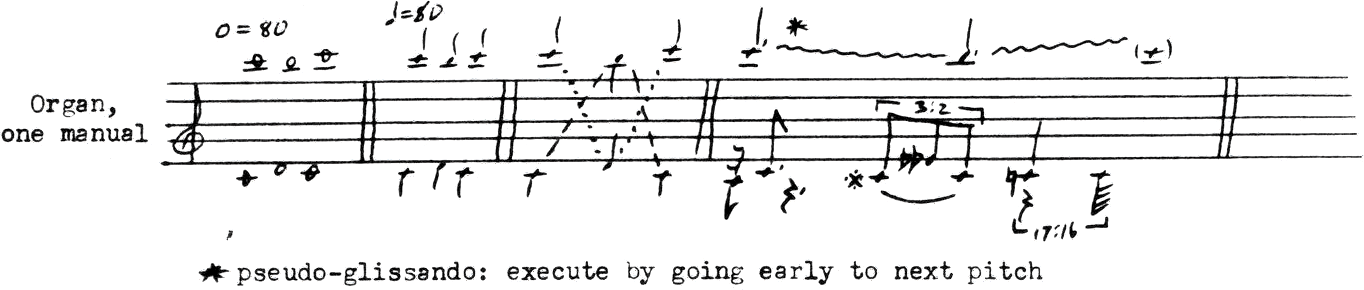
\includegraphics[width=4in]{img/structure_art}\par
}

In each example, the actual sounds, the body of material, is exactly the same. 
The difference is in the different structures defined on the material. The examples 
substantiate my contentions thet the structure is not in the sounds; that the composer's 
analysis of the piece is really a definition and a part of the piece; and that the 
critics' analyses of the structure are definitions attached to the piece, not discoveries 
of intrinsic properties of the sounds. As another example, consider the difference 
between hearing the "Sanctus," \opustitle{Missa Prolationum} of Ockhegem, in no meter (by 
a non-European listener), in one meter (by a lay European listener), and in four 
meters (the intended structure). Arguments such as the one over whether the structure 
of Webern's music is "really" motivic or serial are absurd, since Webern himself did not 
define this point. Many academic structural analyses of art have been irrelevant 
to the aesthetics of the works. 

The purpose throughout all this art is dual; structure or concept art tries to be, 
first, music, visual art, or whatever (which suggests that it is to be listened to, or 
looked at), \emph{and}, something else entirely, to be valuable for its structure or conceptual 
cleverness. Then when the structure is "hidden," "unexperiencable," when it can only be 
appreciated by reading the "analysis," why put emphasis on the body of sound, light, or 
whatever, why listen to structure music, why look at structural visual art, why even call 
them "music," "visual art"? Why not throw away the bodies of sound, light, or whatever, 
and keep the "analyses" of the structure as the works of art? In general, logic, and 
experience (with the results of the artists' efforts), show that the dual purpose of 
structure art consists of irreconcilable objectives; that one can be attained only at the 
other's expense. Which objective are the structure artists trying to attain?---they 
obviously have no idea. Structure art represents obsolete, confused categories of 
activities, categories which by now are obscurantist. Structure (or concept) music, 
for example, needs straightening out, first, by ceasing to call it "music," and starting 
to say thet the sound (or activity) is used only to carry the structure or conceptual 
cleverness, and that the real point is the structure or conceptual cleverness---the 
categorization---and then it will be seen how limited, impoverished the structure of 
these productions trying to be music are. When you make the change, then you are led 
to a far more consistent, integral activity, the same one arrived at below through 
a consideration of pure mathematics. Games of intellectual skill such as chess fall 
into this same category; since, after all, they can be regerded as formalist mathematics. 

Neryt I will discuss pure mathematics. Originally, mathematics was a system of 
beliefs, a doctrine, about the entities numbers, points, polygons, and so forth (Pythagoras, 
Euclid, Platonic geometry). As mathematicians became skeptical, and thus less desirous 
of resting the importance of mathematics on the validity of these beliefs, they changed 
their minds about what the purpose of mathematics is. The purpose became for the theorems 
to be true if the axioms are. In the nineteenth century, as a result of e.g. the ideas 
of Riemann, they became unconcerned to claim that their axioms are true. They began 
to say that the value of mathematics is "aesthetic." Here is when mathematics becomes 
a subject for this essay; when it becomes pure mathematics, when its value is not claimed 
to be that of technology or natural science, but rather more an aesthetic value, when it 
becomes "adoctrinal culture." Mathematics becomes something to be considered alongside art. 
When I became interested in contributing to pure mathematics, for reasons of taste I wanted 
to de-emphasize discovery in mathematics, mathematics as discovering theorems and proofs. 
(Such discovery bored me.) The first way I thought of to de-emphasize discovery was that 
since the value of pure mathematics is now regarded as conceptual interest, aesthetic 
rather than scientific value, why not try to make up aesthetic theorems, without considering 
whether they are true. The second way was to find that the conventional claim that 
theorems and proofs are discovered is unjustifiable; I will return to this point later. 
In the twentieth century, as a result of the ideas of Hilbert, and then Carnap, 
mathematicians became unconcerned to claim that mathematical "statements," the 
mathematical object language, are (substantive) assertions having truth value (as are 
English statements). Rather, they are "merely" series of signs formed according to 
certain rules: formalist mathematics. Then my third way of de-emphasizing discovery was 
to open up unexplored regions of formalist mathematics. The resulting mathematics still 
had statements, theorems, proofs, but the latter weren't "discovered" the way they 
traditionally were. 

Now exploration of the wider possibilities of pure mathematics opened up by me 
tends to lead beyond the form of "making statements," "proving," and the like, so thet 
the term "pure mathematics" becomes completely incongruous. The category of pure 
mathematics---a vestige ultimately of the old system of beliefs canonized by Plato 
(hence the form of statements, proving, and the like)---is an obsolete category. My 
contributions to pure mathematics lead to an integral, general activity of which the 
point is categorizations (having the value of being "well-formed"); the contributions 
need to be classified as such an activity rather than as pure mathematics to escape 
confusion, Traditional mathematics (mathematics as discovery), reformulated, explicated 
to take my findings into account, would be an untypical, small but intensively developed 
part of such an activity. 

The proponents of structure art, pure mathematics, and chess make similar claims 
for them. I have mentioned the claims that structure is an objective property of things; 
and that mathematical theorems and proofs are discovered; and there is a similar claim for 
games of intellectual skill. Two important notions associated with these fundamentally 
identical claims require comment. There is the notion that contribution to structure 
art, pure mathematics, and chess requires high intelligence, the discovery of implications; 
the notion of intelligence as the ability to discover implications. Then, there is the 
notion that structure (as in mathematics pre-eminently) is an objective property of things, 
capable of discovery, demonstration, rational cognition---with particular reference 
to language, art, and the like---whereas meaning, expression, and emotion are not. 
(These pretensions are traditionally an essential aspect of structure art, pure mathematics, 
and chess.) Both notions come down to the belief that there can be an objective relation 
between a name and its referents; for example, an objective relation between the 
metamathematical term "true theorem" and certain theorems, or an objective relation 
between "having serial structure" and a body of sound, or between "checkmate" and 
checkmates. As I said, these notions are discreditable, as can be seen from my 
\essaytitle{Philosophy Proper} and \essaytitle{Primary Paradox}. Thus the notion of intelligence, pretension 
of intellectual superiority, as what mathematicians, chess players, and the like have; 
and the prejudice in favor of structure; cannot be defended. It is about time that 
these notions be discarded. 




\chapter{The Collectivity After the Abolition of the Universe and Time: Escaping from Social Science(1996)}
% CONTENTS
% A. Principles of Natural Sociography
% B. Community and Social Causation in Personhood Theory
% C. Inevitable Stages?
% D. Retroactive Signification
% E. Dissolution of Natural Society
% F. Recapitulation

\section{Principles of Natural Sociography}

Let me introduce a new term for the recounting of social phenomena: \textbf{sociography}. Then both Herodotus and Lefebre practiced sociography; but they practiced it in very different ways. We may call sociography before the time of David Hume (or whoever you want) \textbf{legendary sociography}. The modern sociography which Hume and his successors fought to establish we may call \textbf{natural sociography}.

Here I am forced to interject a qualification which gets ahead of my exposition. Ultimately I propose to dissolve temporally rectilinear natural society. For that reason, I cannot ask for the historical references in this manuscript to be taken literally. These references should be understood as headed by the phrase: "as conventional wisdom affirms."

The aim of this reflection is to escape from social science. But many modern intellectuals would say: "We never accepted social science as a real science to begin with. We already showed that social science cannot be a science." Such remarks are massively misdirective. The positivist and literary-irrationalist critics of social science in the universities are loyal to the social \emph{fact base}---and that fact base is one of modernity’s hardest-won achievements. Indeed, modernist relativists are more loyal to social naturalism than they are to physics, not less. As far as I know, there has never been a published challenge to natural sociography. (Aside from the implicit challenge by the rearguard, those who defend divine intervention, astrology, etc.)

Let me ask a heuristic question. What are the conceptual boundaries–in discourse on social affairs–between
\begin{itemize}
\item the common-sense notion of the world
\item theoretical conceptualization?
\end{itemize}

Social existence "already" involves conceptualization, even before philosophical thinking enters the picture. If we were to invoke ancient evidence (which I am not especially interested in doing), we would find striking examples of how social discourse is conceptualized over and above common sense. Ahistorically, notions of political legitimacy and of law transcend narrowly circumscribed common sense. Kinship. Family law. Property and contract as juridical concepts. Monetary measure of the value of goods. (Whether monetary capital is productive does not have a common-sense answer, as any student of capital theory will know.) The rest of this section will heed these considerations.

Natural sociography adheres to the following principles.
\begin{enumerate}[label=\alph*.]
\item The social collective excludes souls of deceased relatives, not to mention superhuman beings.

\item The social collective excludes animals. Animals enter sociography only as prey and as chattels.

\item All miracles in social records (occurrences precluded by modern scientific laws) must be repudiated.

\item All apocryphal occurrences in social records must be exposed and repudiated.

\item Supernatural causes of human events must be repudiated.

\item Reincarnation is not permissible as an explanation of individual "personality." That means that the Tibetan explanation of the Dalai Lama must be stripped from "real" sociography.

\item Careers in the afterlife (Egypt, Tibet) must be repudiated. Thus the most obvious productive activity of ancient Egypt (and China), the building of furnished tombs for royalty, must be judged a societal insanity.

\item All human needs and wants are posited as mundane, and involve opulence and pleasure. (Power and glory are also conceived as needs; but it is basically taboo to theorize about them.)

\item The concept of destiny, the future as cause of the present, is invoked by some authors–but it is not proper science.
\end{itemize}

All the while, there are certain immaterial ontologies which social science must embrace. Each of the multitude of individuals has a mind–notwithstanding that your mind is unobservable by me. Each individual engages in choice-making. (Various schools of psychology reject this as superstition; but to strip the subject-matter of mentation and choice-making would be intolerably reductionist.)

Humans exist in a culture-saturated realm; which means a realm filled with evidence which can only be appreciated via interpretation. (Inscriptions; pictures and images; etc. etc.) A key issue at every turn in social existence is legitimacy: why, after all, should one cooperate with (or submit to) governmental authority; why should one consent to offered terms of livelihood; etc. etc.? All of this utterly transcends physics and biology; the latter sciences have no basis to investigate these dimensions.

Sociology requires the crystallization and "evolution" of polities to be given a causal rationale which is not supernatural. Even though the individual is the atomic agent in society–a tenet at the foundation of bourgeois economics–his or her consciousness is causally insignificant in comparison to "conditions." Sociology is a phenomenology of political life which

i) treats states as units, as systems;

ii) attends to law;

iii) attends (to a lesser extent) to coalescing and motivating mythologies and rituals.

If sociology wanted to proceed like a natural science, it would have to abstract from concrete phenomena to obtain ideal elements which can have multiple instances. (That is what a scientific law presupposes.) However, history inherently finds its events to be individual. Abraham Lincoln was not an instance of an abstraction which can be repeated at will (as in a series of experiments). Nonactual possibility in history is extremely problematic. (Would Napoleon have commenced such-and-such a battle if he had not had a toothache?) Does sociology seek laws–on a timeline of unique events?

Sociologists indeed require the polity to be a natural system which obeys "socio-natural" laws. For some, the polity is referred to physics and biology as primary realities. At the same time, sociology rests on a modern common-sense notion of the human collective, consisting of an awareness of people one never meets, and some notion of one’s connectedness to them. Again, such information cannot be provided by physics and biology, which do not recognize the existence of individual minds, choice-making, culture, or legitimacy.

Some philosophers of science find a way for a unique human event to express laws. The event, although unique, belongs to a species for which an idealizing, quantifying, experimental science exists. If a great king dies from a heart attack, or from being thrown from a horse, heart attacks or injuries from mechanical shock are explicable in medical biology. [But to say that that is known to be the complete explanation is highly tendentious.]

If, on the other hand, one wants a law which says that "African socialism" could not possibly have worked–because it is not possible for a polity to skip the capitalist stage–then the law would be specific to social process: and the above solution would not help.

There is an opportunity to be far more trenchant here. Physics proposes to provide: an exhaustive account of what is not (nonactual possibility); combined with a voluntary "trifling with nature" called experiment. But concerning our lives and history, we do not want exhaustive accounts of what is not.–And the purpose of our choices is not to "trifle with nature" but to become this person. Actually, why wouldn’t existential self-actualization and scientific experiments have the same character–as choices?

Moreover, if human affairs comprise a unique actual career, then inanimate nature should also comprise a unique actual career.

How is it that modern thought conflates instrumental choice-making with The Order Of The Universe–and then turns around and segregates this package from existential choice-making? When it comes to summing the universe and human life–and to detecting nonactual possibility or not detecting it–modern thought is a shambles.

The prevailing culture tells us over and over: physical science is in good order; whereas social science is suspect (or has not yet proved itself). But nothing requires us to accept this separation of a tractable problem from an intractable one. Like a mantra, they keep repeating "all of it is nature." But then "the problem of knowledge" ought to be a single topic. When, in the name of "nature," modern thought gives us realms which are incommensurate and unsummable, it totally discredits itself.

• • •

B. Community and Social Causation in Personhood Theory

Our field of inquiry is posited to be collective human phenomena. These phenomena manifest intent; and involve meanings (in such a way that to overlook those meanings is intolerably reductionist). In other words, the phenomena involve intentions and interests and ideas. They involve how we conceive or apprehend, understand or appreciate. They involve the appearance of novelties in these respects.

Such (collective human) phenomena are correlative to argumentative discourse.

°

Let us reprise "Personhood II." In the realm of ordinary personhood, other people and culture are palpable to me. Other people and culture jointly constitute the interpersonal arena–or community.

Society is the aggregation which is hypothesized as subtending the (palpable) community. Society is the kingdom, the race, the nation. It is an abstraction, a matter of faith, to which allegiance is demanded by palpable specific people.

So society is a "grandiose Other." A grandiose Other is advanced as the ultimate source of meaning, the ultimate source of my emotional gratification and judgmental self-consciousness. At the same time, the grandiose Other is primarily speculative, and outside "my ostensible world."

The universe of physics (called Nature) must be mentioned in this connection as hypothetical, inferential, derived, and grandiose–as a modern god. The enshrining of Nature as a god is a precedent for the modern enshrining of society as a god. The physical universe is not claimed to be a source of meaning, however.

In modern culture, the grandiose Objectivity which has priority is (to repeat) society. Society's claim on us as persons (even when we are treated as pawns) is far broader and more important than the physical universe's claim on us. Typically, the primary avowed loyalties in modern culture are to society.

Extending from one's emotional involvement with other people, society becomes an object of one's passionate belief. The hypothesized abstraction seems to be a living presence: as when people march off to war for The Nation–or dramatically refuse to do so. "Attachment" makes society more compelling than the physical universe. Because society is an object of passionate belief, because it becomes a hallucinatory living presence, it cannot be sharply distinguished from community (which is palpable), even though it remains impalpable (a hypothesized abstraction). So society has a close and compelling connection to the palpable phenomena of other people and culture.

At certain points, personhood theory passes to a higher level of credulity and integrates its analysis with one of the preexisting hypotheses which it has discerned. This is what happens in the case of culture. Personhood theory pictures my cultural competences (e.g. English orthography) as deriving from society. Namely: culture is that palpable aspect of society which is interior to me and at the same time is an externality broader than other people as individuals.

Recognizing how close society is to community in belief, I propose to be flexible with regard to whether the person is conceived in a communal or a social context.

The community confronts me with symbols and offices which imply an organized collective, legitimation, manifestations of a group will, etc.

One cultural phase of community life includes the community's "tradition," symbolism, ritual, etc.–all of which are emotionally charged. This phase must be considered one source of my emotional sensitization or capacity.

The community may force upon me a significance, and an assortment of privileges and disadvantages–so much so that I am forced to carry out this "imposed social role" or to grapple with it. The role may place me in competition or conflict with other people. I can also be gratified by the celebration in ritual of my imposed status (although I do not earn this gratification).

I have a greater or lesser degree of autonomy, relative to the community, in respect to being supplied with pursuits and goals, and in respect to making judgments of every sort.

I can obscure my choice-making by becoming a vassal of "society"–of a legitimated organization or institution.

I may engage in a pursuit which I suspect to be dishonest or otherwise contemptible because the community approves of it. Of course I do so to gain tangible rewards, in analogy with knowingly deceiving another person to benefit myself. But something beyond my craftiness is involved here. I maintain a knowing self-deception and vassalage in which legitimacy means more to me than sincerity.

The interpersonal arena is a source of meanings to me. My connections to the interpersonal arena in regard to praxis, emotional sensitization, indoctrination, etc. have an effect on my sense of sanity, my personal identity, my level of fulfillment, etc. Thus, the interpersonal arena can be a source of skills worthy to be sustained and regenerated. It can also be a source of acute dilemmas and destructiveness impinging upon me. In either case, the interpersonal arena is a source of problems and missions.

Moreover, the problems and missions can appear in my consciousness as consequences of my skills. Having been indoctrinated with little choice in the matter, that indoctrination now surfaces in the guise of my skills, for one thing. (Examples at the level of the present discussion are language use, mathematics, music, profit-maximization.) If I do not consciously review my indoctrination, then I will carry it with me by default. Moreover, my private and idiosyncratic dilemmas with natural language, with mathematics, with art, with profit maximization, etc.–and my private and idiosyncratic ventures in these fields–can represent vital dilemmas and ventures for the interpersonal arena.

But the community's destructiveness or bankruptcy may consist precisely in its inability to embark upon vital ventures–and in its fostering of individual pursuits which disregard and exacerbate its dilemmas.

I can undertake a vital venture or address a vital problem; or I can avoid doing so. And I can belong to a community which wants such a task addressed; or to a community which discourages attention to such a task. The possible ramifications of the community attitude, for my judgment of myself, are complicated. Inner pride or lack of it can run counter to express community approval or contempt.

°

Social role can submerge a person. More accurately, the social role can be said to fixate the individual to mutilated perception. But I then say that the social role is a sort of ideology and skill which the individual is fixated to. The submergence of the person by a cumulating social role is an outcome in which the person is guaranteed to be traumatized, stigmatized, impaired, truncated.

Certainly, in some cultures or communities, socially acclaimed and validated roles can also allow intrinsic splendor. Even so, we must not allow the doctoring of sociography (at the level of renowned individuals in history, for example) to obscure the fact that these socially approved achievements had great difficulty coming to the surface in the first place–and that they were subsequently dishonored by deteriorating communities.

But to exist in fixation to a cumulating social role is always a depersonalized, mythified existence–even when it is producing useful output. Of course, being submerged in a social role is only one of a number of ways in which existence can be depersonalized and mythified.

My formulations give social role–or thematic identity–or imminent character–the guise of a self-caused cause or looped cause. The circuit of attachment through the person-world is not a linear causal phenomenon; it is a phenomenon of scrambled or turbulent causation. It is a dynamically balanced confined turbulence. What is awful about being submerged by a social role, in the cases known to me, is precisely that such submergence is self-reinforcing.

In "Personhood II," I had a reason for focusing on certain "ruinations" which individuals underwent. First, an ahistorical illustration. The culture may mutilate a child's faculties and inculcate him or her with debasement–without pushing the child to the point where he or she demands escape as a right or becomes a precocious social critic.

We again encounter the social doctoring of sociography–this time at the level of individual longitudinal records. Children do express distress, they do demand escape as a right, they are precocious social critics until they are subjugated. Higher and higher tolerances for anguish, or compensating rewards, have to be developed. In due course, the child begins to perpetuate the stigmas in him or herself. At the least, he or she acquiesces; at the most, he or she may become a well-rewarded advocate of the community.

A case at a different level is specific to America and the U.K. in the second half of the twentieth century. The Seventies saw the explosion of cults and ritualized degradation in America and the U.K. Then, in the Eighties, the American Establishment launched a campaign to win back the middle class; and it became fashionable to be a Yuppie. When the recession occurred at the end of the Eighties, the Yuppie role became tarnished. So social history is superficially changeable. These ebbs and flows are not the level I should address. What we should glean in this connection is that the cults and the ritualized degradation signal the long-term trend of techno-capitalist civilization.

I include these remarks on the doctoring of sociography, and on the civilization’s trend, to illustrate how early personhood theory arrived at hypothecations about society.

°

The person submerged by a social role emerges as a person who is "done to." On the other hand, in a tiny minority of cases, we have the emergence of person who "does" or "does to." Why, then, is a given person one way or the other?–and can he or she be switched from one type to the other?–and does a person who is always one type nevertheless have a potential for the other type?

Let us work through the notion of society’s imposition of the individual’s identity. Medieval serfs were illiterate and never saw money in their entire lives. Today their descendents in Western Europe all read, possess money, and spend money every day. The reason why serfs did not learn to read or to allocate money was that (in effect) they were not recruited and given cultivation to these ends.

There is a view which would say that the serfs, as a multitude which had been assigned the same fate, became aware that they were being taken advantage of in a common way, and fought for the cultivation (schools, etc.) which they subsequently received. This is not false (the French Revolution); but it is misleading in the extent to which it makes the serfs into autonomously rational protagonists. It does not take into account that the descendents of the serfs remained outside the controlling class–that the "toilers" have never commanded the system. The collapse of the workers' paradises makes this observation all the more decisive.

It is more realistic to say that advanced capitalism continually revolutionizes technology and continually erases and replaces social relationships. (Capitalism also spurs developments such as the dissolution of the nuclear family, and feminism, which the Establishment did not calculate.) So the aggregate displays a rationale which overrides the individual.

That is why the achievements and satisfactions which are possible to people are seen as results of how much cultivation the Establishment gives them.

But in personhood theory, the question of why people are what they are focuses in a different way. The topic was anticipated in sections of "Personhood II." The sociological perspective is tacitly dedicated to a doctrine of underprivilege and socially engineered redemption. Somehow that mind-set fails to engage our announced problem. Let me present a shock-question to clarify the issue.

Would a Nobel-prizewinning physicist agree

that he believes physics because his naivété

was exploited by malicious elders, because he

was crushed by his elders, because his elders

did not give him enough cultivation?	

The sociological perspective–in the name of recognizing that the serf's backwardness was imposed from without–treats the serf's effects on other people as if they were imaginary or didn't matter. It treats the serf's choices and life as if they were tuberculosis–a fatal disease which a few pennies' worth of medication could have cured.

Capitalist technology and centralization have created the possibility of imposing changed fates on entire populations. A member of the administrative class can regard all the choices and lives of a population as a reversible condition. Then people really are what the administrator chooses to make them by pushing this or that button. People are so thrilled by the prospect of human manipulation on this level–or by the prospect that the Establishment is due to give them cultivation–that they overlook that the sociological perspective makes all their choices and their lives chimerical (or revocable). "You did it because you were programmed improperly." How do you choose and act if you believe that your choices and actions have the ontological type of a disease, an error in past programming? And who says that the serf's life was "bad" or unnecessary? And yet people have learned to think in these terms–to want to be told that what their betters permit them is what they are.

A novelty may arise in how we conceive or apprehend, understand or appreciate. That led me to the notion of an unprecedented fate–of a person upholding an authentic identity-theme coming from the future. Such a person emerges as a person who "does" or "does to." Section D is devoted to this topic.

The ambition to transfer social engineering to seriousness and originality, by vaccinating people with seriousness and originality, is an ill-conceived ambition. Seriousness and originality are not "done to"; they "do (to)." They are not implanted. They appear unpredictably. (Of course, my attempt to assert my sincerity and to make the interpersonal arena conducive to it may reawaken seriousness and originality in another person.) I speculate about the authentic identity-theme which comes from the future: to show that one need not assume the social engineers' cause-and-effect. One does not even have to believe that "solutions" are fabricated from past to present.

Given my speculation about unprecedented fates, can average people be said to have routine fates? My considered answer is no. That is because to say that a person fulfills a routine fate cannot be distinguished from saying that that person is determined by the past, by circumstances.

Personhood theory refuses to acknowledge people as objectivities in a deterministic process. (Except to acknowledge that this conception itself is one of the characteristic nonsensical fantasies.) One who adopts the person-world outlook cannot consider his or her choices and life as a reversible mishap. Personhood theory cannot consider palpable choices and lives as chimeras or as revocable.

The demand for a calculus of society is, in the light of personhood theory, an ill-conceived demand. The notion of the authentic identity-theme coming from the future is introduced to show that one need not assume the social engineers' cause-and-effect. We do not even have to believe that "solutions" are fabricated from past to present.

Seriousness and originality cannot be thrust upon any given person by outside manipulation. Metaphorically, escape hatches are opened by the future, as coherent novelty, in conjunction with moments in which choice is forced–moments in which the arena of action might be reconceived, loyalty might be shifted, effectiveness and gratification might be reconceived, etc.

• • •

C. Inevitable Stages?

Marxism proves more decisively and relentlessly than any other ideology that we are robots. It then goes on to say that those of us who are in bondage should be freed. But at the level of the cogency of the ideology, if the slaves are robots, then why must they be freed? (So that there can be an exponential expansion of production? But to what end?) What difference does it make to a robot?

Before my turn to personhood theory, I indulged Marx’s historical materialism as a plausible explanation of the moral codes of past epoches. But this plausible contribution of Marxism has to be reconsidered. Perhaps the succession of stages in history (slavery, feudalism, capitalism) was necessary. But the person-world premise reconstitutes our understanding of what the stages comprised:

realized choice alongside external conditions of the moment;

realized choice and external conditions as equal constituents of a single "world."

It should also reconstitute our understanding of their necessity. The pivotal ingredient in the transition from one stage to another is an imagination and its embrace which have no sociological explanation.

The Marxist-Leftist tradition shares presuppositions of the modern Western culture of which it is a variant: blind faith in natural science; dogmatic materialism; the assumption that natural science and dogmatic materialism are allies of revolution; socio-idolatry.

Marx wanted "revolution" to transform the economic class structure while remaining relentlessly loyal to the scientific world-view. Ironically, this program may be self-frustrating. It may not be possible for a movement which preaches loyalty to the scientific world-view to gain support in late capitalist society for an insulated overturn of the economic class structure. (As I often mention, bourgeois economics has long since rooted itself in physical science.) Capitalism may be able to assimilate to its own fabric any scheme of economic liberation which proclaims the equality of people as robots and commodities.

• • •

D. Retroactive Signification

In rare cases, the individual may "steer" toward an identity which embodies coherent novelty–in that sense steering toward an authentic identity coming from the future. This depends on the earlier principle that the phenomena involve novelties in how we conceive or apprehend, understand or appreciate.

(In the present discussion, I am omitting the analysis which differentiates coherent novelty from the successful individual–from the rewarded celebrity. Today, the case has come to the foreground of a "creative submission" which is a compensatory experience of license, irresponsibility, puerile or malign misbehavior, etc. After all, criminals such as Manson become heroes; people live vicariously through them. These episodes are not what I mean by coherent novelty.

My psychology is inherently an introspective inquiry. Another principle is required which I do not expound here. The reader has to classify him or herself. The dishonest reader cheats him or herself, no more and no less. All these supporting principles are discussed in my depth psychology or in person-world analysis.)

The notion of steering toward an identity coming from the future belongs in a reconstituted discipline of psychology. All the more so because the problem of predicting individual outcomes has received so much attention in psychology–not only in the highly professionalized field of psychological testing, but in impromptu and unwritten appraisals made by psychoanalysts, etc. In turn, there are repercussions for the notion–so characteristic of sociology–that the individual’s identity is an imposition by society. There are repercussions for the notion that greatness is a gift which society gives to the individual; and there are repercussions for the interpretation of the metamorphosis of societies.

Retroactive signification means that a notion of deterministic evolution fails because of the emergence of coherent novelty. Even a liberal version of the scientific method, extrapolated to socio-psychology, would not be able to predict what certain people would become: because what they would become would in fact displace the reigning hermeneutic with an unprecedented hermeneutic. In other words, science would have to applaud its own death in order to predict the outcome.

To use the surprising outcome to upgrade the "laws" by which you analyze the "initial data" would deprive us of the lesson which the phenomenon affords. The earlier period’s "ignorance" is an essential feature of the realm being studied. It’s not scientific ignorance in the sense of lack of enough data-points to fit the curve. What the future brings are knowledges which blow up the scientist’s entire "personality." Faculties that the earlier scientist doesn’t have; successes that crush him as a person. The outcome exposes his life as a lie or sham. He is caught worshipping the wrong god.

This means that the locus of retroactive signification in the first instance is one person’s life: a course which is inherently individual, and which involves interests and ideas which fragment, conflict, and unite. The subject-matter is inherently about the antagonism of ideas and interests, about antagonisms in what anthropologists call culture. Retroactive signification is "psychological" and interpretative.

In the perspective of retroactive signification, only the future can teach the scientific observer what the past meant. He or she couldn’t have made an analysis of the past on past evidence which would have divined where it was going. It is impossible to know what the initial data mean when they appear. They are the germ of something incommensurate with his or her framework for appraisal.

The scientist of the later generation responds to coherent novelty by "growing" a new sort of "personality." He sees, in the past, what a past scientist could not have seen even if more "facts" had been provided.

That is not to say that the notion of the window to the future does not have risks–which I will note as I proceed. Why wouldn’t we blame Marx for Stalin, or Jesus for the Crusades? Here there is an answer: our interest is in the genuinely novel idea which arises. That this idea is put to use by selfish or psychopathic interests is important to the casualties–and to the historian–but does not prove that selfish or psychopathic aggression stems uniquely from the idea in question.

°

Can the notion of destiny, here called retroactive signification, be aggregated–applied to social totalities? I found retroactive signification to be almost vanishingly rare. It played the role of an exception to our much more usual apprehension that society shapes the individual.

I asked, earlier in this manuscript, whether average people could be said to have destinies which, since they are not awesomely surprising, should be called routine. My considered answer was no. To say that a person consummates a routine destiny cannot be distinguished from saying that the person is determined by the past, by circumstances.

History does not give us the same opportunity to contrast the rare outcome with the commonplace outcome that a consideration of individuals does. If one imagines that the rise of modernity in Europe was a rare outcome relative to societies which could be considered static or essentially repetitive, nevertheless modernity became prevalent and did not remain an individual possession. If modernity spreads and affects everybody, then it is indistinguishable from a Marxist "stage," or from a stage of civilization.

The rare individual’s "career" brings forth a coherent novelty which changes the basis of "knowing." Let me first clarify the connection I make between crystallization and "the future." The novel identity progressively focuses–in an individual life. That led me to say that it comes from "the future." Actually, there are cases in which the person focuses, but the public does not respond. John Philoponus. It took one thousand years for his work to be redone by successful men, and 1500 years for him to become famous.

I am suspicious of transferring the notion of an individual life-course to society so that we have the notion of a society’s career. Nations do not have selves; they are already chimeras.

The difficulty is not that there are not candidates for coherent novelty at the level of societies. [National cultures are such candidates.] Rather, a new liability appears. I was willing to recognize contributions from individuals which were diverse and relative. If we do that at the level of nations, we end up lionizing those myths which became successful. The subjective moment is lost, and all we are left with is a dominating myth. There is nothing wrong with it, except that it has lowered the discussion to the level of social history or history-of-ideas. Then we get involved with chauvinistic triumphalism.

Again: there have been many novelties at the level of national cultures which were underestimated by Establishments. But there are arguments against assigning destinies to national cultures:

1) Societies don’t have selves.

2) To recognize diverse and relative contributions at the level of societies can only mean taking successful myths as the topic.

Suppose we assume that European modernity is the fruition of humanity’s existence. To surround modernity with congratulation is dubious, since modernity brings terrible penalties from which we need to be rescued. Another profound difficulty: modernity’s judgment of the meaning of an earlier age is not necessarily worth more than that age’s own judgment of its meaning.

A major lesson emerges here. The perspective of retroactive signification is always discarding the past as merely anticipatory. But isn’t that too triumphalist? Past eras had their own values–which the future may not improve on.

When the future has the character of a regression to the status quo ante (as it often does)–possibly combined with a displacement of society’s preoccupations to other axes of antagonism–then the notion that this outcome consummates a destiny is disappointing. When the future can be conceived as a regression or mere displacement, then the future’s judgment of the past’s meaning can be a retreat into retardation. (Philosophy’s judgment of Hume, which regressed from his achievement.)

Is modern natural science the fruition of Greek natural philosophy? The trouble is that we may learn far more from Aristotle if we do not simply read him to see where he agreed with "us."

Ancient Judaism was underestimated by pagan élites, and so presaged coherent novelty. But what was its fruition? There is not a unique answer. To give an answer will almost automatically be invidious; unless we confine ourselves to commonplaces about the generic influence of Biblical religion. Again, that is a theme for history-of-ideas or social history.

Again, to apply the notion of destiny to society would only converge with Marx’s stages of history or with history-of-ideas. Surely retroactive signification’s liberating implications lie in a different direction.

°

Sociology has promulgated the cliche that society shapes the individual–or even that the individual’s identity is an imposition by society. Retroactive signification is credible in the individual life: that militates against sociological causation of the individual. A reconception of the way the individual is "inlaid" in society is demanded. Recall that one’s private conflicts over the skills with which one has been indoctrinated can evince vital dilemmas and vital ventures for the interpersonal arena.

Sociological causation of the individual is impressive only to the cynic. Personhood theory refuses to acknowledge people as objectivities in a deterministic process. One who adopts the person-world standpoint cannot consider his or her choices and life as a revocable mishap. Personhood theory cannot consider palpable choices and lives as chimeras–or as revocable.

In the rare case that one's authentic identity-theme comes from the future, guiding oneself toward it remains a matter of pronounced willfulness in a context of uncertainties. It is possible to drift rather than to push toward the distant identity-theme. And subjectively I often have to gamble–even if my purpose remains fixed. (By upholding or relinquishing the identity-theme from the future, one guarantees or nullifies it as a future?)

The scope of "choice" includes the possibility of shaping your loyalties. Such shaping of loyalties covers

–reconceiving effectiveness and gratification;

–reconceiving the purpose of life;

–reconceiving the arena of action.

In speaking of altering your loyalties, everything up to and including the determination of reality is open. When the individual is being "attracted by" an unprecedented fate, choice in a moment of crisis can be seen as a phenomenon in which the remote future contacts the present. The crisis gives one some choice over the way one's distant future shapes one's present.

The "career" which is interpreted as retroactive signification is correlative to seriousness and originality–and seriousness and originality cannot be instilled by outside manipulation. In turn, whether the individual will be cognitively protean, which is what I wanted to know, presumably depends on seriousness and originality.

Because we are talking about a novelty which depends on vital dilemmas for the collectivity which the collectivity doesn't acknowledge, the person who expresses the novelty refuses the depersonalization of social role.

• • •

E. Dissolution of Natural Society

Let me now consummate the dissolution of natural society and its rectilinear career as an ontological category. Drawing on previous writings, I sketch a hypothetical civilization outside the plane of natural society. [That means appealing even more urgently to personhood theory.]

In this hypothetical civilization, the collective can freely change the laws of nature. That presupposes claims, made previously and elsewhere, that scientific reality can be superseded. There is a dispelling of deceit and gullibility, concomitantly with the awakening of faculties, and with emotional sensitization: yielding intellectual techniques which supersede the compartmentation of faculties characterizing the present culture. Thereby, new mental abilities are invented. The community is open to avenues of metamorphosis of the life-world. The comprehensively assembled "meta-technology" would be self-conscious about the inherited view of factual reality, going beyond it in an operative way. Again, my perspective is that of a novel arena which outruns what was formerly considered factual reality. (My meta-technological writings, etc., are a prerequisite for understanding the terminology of the requirements to follow.)

The envisioned mode of life invokes dimensions of human potentiality which hitherto were supported only by different cultures. I'm seeking a unitary experience which transmits many dimensions of potentiality.

My interest here is with the ramifications of these claims for interpersonal life. If meta-technology could be implemented collectively, we would accede to an uncanny life-world. To express the matter from a present-day standpoint, the new mode of life would be a waking-dream reality or enchanted reality.

In order for a collective to be able freely to change the laws of nature, all persons would have to have parity of "station in life" and parity of authority in the culture. Moreover, the total of menial and routine labor would have to decrease to the vanishing point.

Let me consolidate here all the consequences of direct import for the present discussion.

×	One intellectual consequence is that the realism of history would be placed in suspension. The higher civilization would consign history to a lesser grade of realism. The supposed edifying effect of history is dispensable. Whereas today, we need to preserve traditional culture as a bulwark against dehumanization by the current culture, the higher civilization would mean a revival of personalistic and hallowed expression, on a new level: "soul" would not longer reside only in old languages, old buildings, old statues, old texts.

From another angle, the motive for people to keep score as to their ancestral status (or lack of it) would disappear. "Consciousness" could break free of its material antecedents (circumstances).

×	The higher civilization presupposes an intellectual defeat for physics; for Marx’s materialism; and for all the doctrines which hold that capitalism is necessitated by physico-biological nature itself. See (A) and (1) below.

×	The new mode of life is not compatible with a social order in which most people are consigned to material servitude. Not only would the sought-for inspiration not appear; the uncanny instrumental activity or meta-technology would not appear.

So it's not like Pakistan and the atomic bomb (or the priesthood in ancient Egypt)–advanced technology coexisting with a population of paupers or slaves. See (E) below.

°

The following principles are requirements–expressed as if from within the new mode of life, in the new terminology. Parenthesized numbers refer to comments on each statement, collected in the following section.

A. The life-world (lived experience) is understood as an integration of:

–substantial, operative interdependencies of awareness and objectivity;

–the conventionalistic grading of experiences (as to "realism");

–logically impossible situations (states of the world)–i.e. situations requiring simultaneous mutually exclusive descriptions in the medium of thought inherited from scientific civilization.

The principle of the personality's orientation in "reality" is: consciously to maneuver through the logically impossible world-states, manifesting instrumental mastery over objectivities inherited from the previous civilization. (I.e. scientific objectivities). (1)

B. The foregoing cannot be achieved merely by adopting a neutral, inert mental state, by positioning oneself mentally relative to propositions.* Sustainable inspiration (exalted centered activation and presence) and uncanny states of consciousness are required.

C. The principles of evaluational processing of experience (or grading of experience) which underlie a novel determination of reality are shared or collective. Only thus can novel determinations of reality be promulgated in the life-world.

D. The novel determinations of reality are linked to emotionally supportive intersubjectivity. Only thus can the novel determinations of reality appeal to a community.

E. The other persons have parity of "station in life" and parity of authority in the culture with "the self" ("this individual," myself). Only thus can they stimulate inspiration and uncanny states in "this individual."

F. The community from which people concretely originate and "learn to feel" becomes the same community that pursues mastery over scientific objectivities and gains an uncanny or ecstatic sense of the world. Inasmuch as the required shared principles of grading experience, and the required intersubjective emotional gratification, connect, a person-configuration freed from demeaned pragmatism is evinced. (2)

G. The individual experiences "desirables" as qualitatively specific.

H. The individual insists on the satisfaction of the qualitatively specific and unequal needs of self and peers for the material requisites of life. (To recognize inequality of individual needs does not mean endorsing different grades of reward. To resolve competing claims, a representative body is needed.) (3)

I. Production of the material requisites of life is planned by a representative body to shrink necessary labor time. (Automated collectivism.)

J. Individual and the collective entertain spontaneous "amusement" or "play" ("brend"), without seeking to displace or objectify it.

K. Sensuous-concrete vehicles for the collective expression of exalting values are encouraged.

L. Individual and collective are receptive to future novelty which is unpredictable and incomparable and yet is coherent or thematic. (4)

°

Next, the commentary, which is expressed in the old terminology.

(1) Self-subsistent objectivities, and affirmative consistent theories, would no longer be sought as foundations of reality. As far as the physical world is concerned, a fragment of what I envision is provided by my "Superseding Scientific Apprehension of the Inanimate World: The Phenomenological Basis of Physics" (1990).

(2) Here uncanniness and ecstasis are positioned as notions reactive to everyday banality. In the new mode of life such counterposition would no longer be necessary.

(3) This statement on satisfaction of needs is pertinent so long as a separate sphere of material requisites of life can be distinguished.

(4) To the present civilization, the new mode of life would seem a waking-dream-reality or enchanted reality.

\visbreak

F. Recapitulation

Let me try again to specify the object of social science. A world-wide aggregate of humans on a geological or biological time-line whose future is determined by efficient causation. No author but me would remark that this object is a phantom. Nonetheless, the urgency of rotating out of social science stems from considerations in lived experience; considerations which envision a novel existence whose preconditions have begun to be worked out in theory. These are concerns unique to me which have occupied me for many years.

The exposition is rambling and not yet sorted out. (That applies especially to the overhanging progressivist identitifcation of ‘futural’ with ‘superior’.) But never mind that. The "society" discerned by social science is a hypnotically instilled hallucination. The notion of causation which subtends it is humiliating and enslaving. I have exposed crucial junctures at which sociological causation–deeply plausible though it may be–is annulled. Beyond that, there comes a point in historical time at which the historical time-axis evaporates. The collectivity awakens from, outgrows, the imaginary order with which it had surrounded itself.

\end{document}
